% web10 paper — FOURTH DRAFT: a clean resynthesis from shot 0 (the 12 beats
% + the monetization beat) told through the figure set. The operator's
% call, 06.11.2026: the third draft "inherited the junk from the other
% papers" — the entry (the email door), the formal apparatus (the two
% trust-wall tables, the set expressions, the principal classes), the
% implementation-status hedges, the heavy related work. None of that is
% in this draft: the manuscript is the beats, the figures are the map,
% the evidence is carried as fact from the records (craft/evidence.md).
% Page budget: lifted (operator, 05.11.2026) — complete over concise.
% Render: tectonic main.tex  (from this directory)
\documentclass[sigconf, nonacm]{acmart}
\settopmatter{printfolios=true}
\AtBeginDocument{\addtolength{\footskip}{36pt}}

% --- packages (all in the tectonic bundle) ---
\usepackage{booktabs}
\usepackage{enumitem}
\usepackage{microtype}
\setlength{\emergencystretch}{2em}
\usepackage{xcolor}
\usepackage{listings}
\usepackage{graphicx}
\usepackage{tikz}
\usetikzlibrary{positioning,calc,arrows.meta}

% Brand tokens (knowledge-base/strategy/design.md §13)
\definecolor{web10bg}{HTML}{09090b}
\definecolor{web10fg}{HTML}{fafafa}
\definecolor{web10brand}{HTML}{8b5cf6}
\definecolor{web10brand300}{HTML}{c4b5fd}
\definecolor{web10muted}{HTML}{27272a}

% Pin implementation links and source-size accounting to the reviewed snapshot.
\newcommand{\artifactbase}{https://github.com/jacoby149/web10}
\newcommand{\artifactrev}{317fa349eae714ddde07f249ca65cdaa34b6459b}
\newcommand{\artifactdir}[2]{\href{\artifactbase/tree/\artifactrev/#1}{#2}}
\newcommand{\artifactfile}[2]{\href{\artifactbase/blob/\artifactrev/#1}{#2}}
% Domain prototype: immutable tested code/receipt publication, separate from size snapshot.
\newcommand{\domainartifactrev}{26720acba859c7eb03fc5d26a6221cdde5b764a1}
\newcommand{\domainartifactdir}[2]{\href{\artifactbase/tree/\domainartifactrev/#1}{#2}}

\lstdefinestyle{sql}{
  language={},
  basicstyle=\ttfamily\footnotesize,
  breaklines=true,
  frame=single,
  framesep=4pt,
  rulecolor=\color{gray!50},
  backgroundcolor=\color{gray!6},
  keywordstyle=\bfseries,
}
\lstdefinestyle{json}{
  language={},
  basicstyle=\ttfamily\footnotesize,
  breaklines=true,
  frame=single,
  framesep=4pt,
  rulecolor=\color{gray!50},
  backgroundcolor=\color{gray!6},
}

% --- acmart metadata ---
\setcopyright{none}
\acmConference[SIGMOD 2027 Industry Track]{SIGMOD 2027 Industry Track}{}{}
\acmPrice{}
\acmISBN{}
\acmDOI{}

\title{Your Data, Your Rules: \\ Extending the Decentralized Web}
\author{Jacob Hoffman}
\affiliation{\institution{web10 Inc.}\country{}}
\email{jacob@web10.app}

\begin{document}

\begin{abstract}
What makes your data worth owning is the graph around it: who follows
you, who belongs to your groups, who you have allowed to read what.
The content is portable in principle; the social graph---the follows,
the groups, the audience---and the rules that go with them are the part
no platform lets you keep. \textbf{web10} is a deployed, user-addressed
data platform that closes that split: the access rules are your own
data---grants are rows in the very store they protect---and a second
application reads the first's data with per-service grants, finer than
OAuth 2.0. A new read pattern is a new query, not a new backend. Your
audience travels with you: an address is a domain you own, a node
verifies but cannot control, and public subscriptions outlive a provider
change. The platform takes no cut---creators keep 100\% of their
monetization, and nodes compete for them on terms, not leverage. At the
bottom, ClickHouse at scale: at 1,000 followed creators, the cost lives
in the access layer, not the database (7.64\,s to 363\,ms). When the
data leaves a node, the rules leave with it.
\end{abstract}

\maketitle
%=============================================================================
\section{The split every platform inherits}
\label{sec:intro}

What makes your data worth owning is not the content. It is the graph
around it: who follows you, who belongs to your groups, who you have
allowed to read what, and what each of them can do there. The content is
portable in principle---a post is a post---but the social graph---the
follows, the groups, the audience---and the rules that go with it are
the part no platform lets the user keep.

The systems the reader knows as ``the decentralized web'' each moved a
piece of that. Solid~\cite{solid2016} decentralized the \emph{store}:
one pod per user, the data in the user's hands, encrypted and
pod-bound. Mastodon and Bluesky decentralized the \emph{transport}:
federated content between servers, and on Bluesky the choice of relays
and app views with it---user agency and provider switching
\cite{kleppmann2024}. Every one of them left the access layer in the
platform: who follows whom, who may read what, who belongs where, and
what a second application may do with the first application's data are
still decided by backends and object models the platform owns
\cite{activitypub2018}. The content travels between their systems; the
permissions do not.

\textbf{web10} closes the split. It is a deployed, user-addressed data
platform: the node that hosts it is completely generic---read and write
on data, and configuration for identity and access, executed every time
the data is used---and the access rules are the user's own data, in the
very store they protect. A social application, a snake game, and a
marketplace run on the node and interoperate on shared data through the
same boundary: the game and the marketplace read the social
application's \texttt{profile} documents with no node change and no API
agreement between the applications (\S\ref{sec:extend}).

The contribution is a combination, and no part of it is new:
user-owned storage, user-managed grants, and application-written queries
over authorized relations are each established ideas
(\S\ref{sec:positioning}). What no prior system we compare carries is
the conjunction---all three, on one shared columnar store, with the
access decision made on the input before any data moves. Five
properties, and this paper closes on each:

\begin{enumerate}[leftmargin=*,nosep]
  \item \textbf{User-owned, portable data, all formats.} A post, a
  profile, a game score, and a marketplace listing are documents in the
  same store, differing only in the service string and the JSON shape
  the application agreed to use (\S\ref{sec:store}).
  \item \textbf{Fine-grained, user-managed access.} A grant is a row:
  principal $\times$ group $\times$ service $\times$ operation;
  publicness is a grant, not a flag; the end user runs the IAM
  operations a cloud operator would express as policies, over their own
  data (\S\ref{sec:access}).
  \item \textbf{Cross-node-addressable access.} A principal is
  \texttt{provider/\allowbreak username}, globally unique across the
  federation; a foreign token is verified, not registered---one cached
  \texttt{/certify} answer, the same access check on every read
  (\S\ref{sec:network}).
  \item \textbf{Composable, app-defined queries.} The node has never
  learned a social concept---no posts table, no feed endpoint, no
  followers construct---and the query boundary keeps the shared store
  sound: the reader's readable set is compiled into the query before any
  data moves (\S\ref{sec:boundary}).
  \item \textbf{A user-addressed network without federation.}
  Sovereign nodes, client-mediated reads, no central authority, no
  shared database; an address is a domain the user owns, and the
  audience travels with it when the account moves (\S\ref{sec:network}).
\end{enumerate}

The evidence is connected, bounded, and named (\S\ref{sec:evidence}):
a game and a marketplace reusing the social application's data through
a real browser's consent and revocation; a grant that crosses a node
boundary and is
revoked at the owner's node; a public subscription that outlives its
provider; and a measurement that found where the access layer's cost
lives---7.64\,s to 363\,ms at 1,000 followed creators, with the
one-group counterweight in the same trial.

Figure~\ref{fig:app-arch} draws the system the paper walks through: the
application's data layer in the browser, the thin generic node, and its
two stores---with the messages that move between them.
\S\ref{sec:access} states what the node is and why the rules are the
user's data; \S\ref{sec:store} the store at the bottom and the fork
Solid did not take; \S\ref{sec:boundary} the query boundary;
\S\ref{sec:extend} how an extension costs a role and a policy;
\S\ref{sec:network} the address, the handshake, and the domain;
\S\ref{sec:money} where the money flows; \S\ref{sec:lessons} what
running it taught; \S\ref{sec:evidence} what was measured;
\S\ref{sec:positioning} where the combination sits against the systems
it combines; \S\ref{sec:concl} closes.

\begin{figure*}[t]
  \centering
  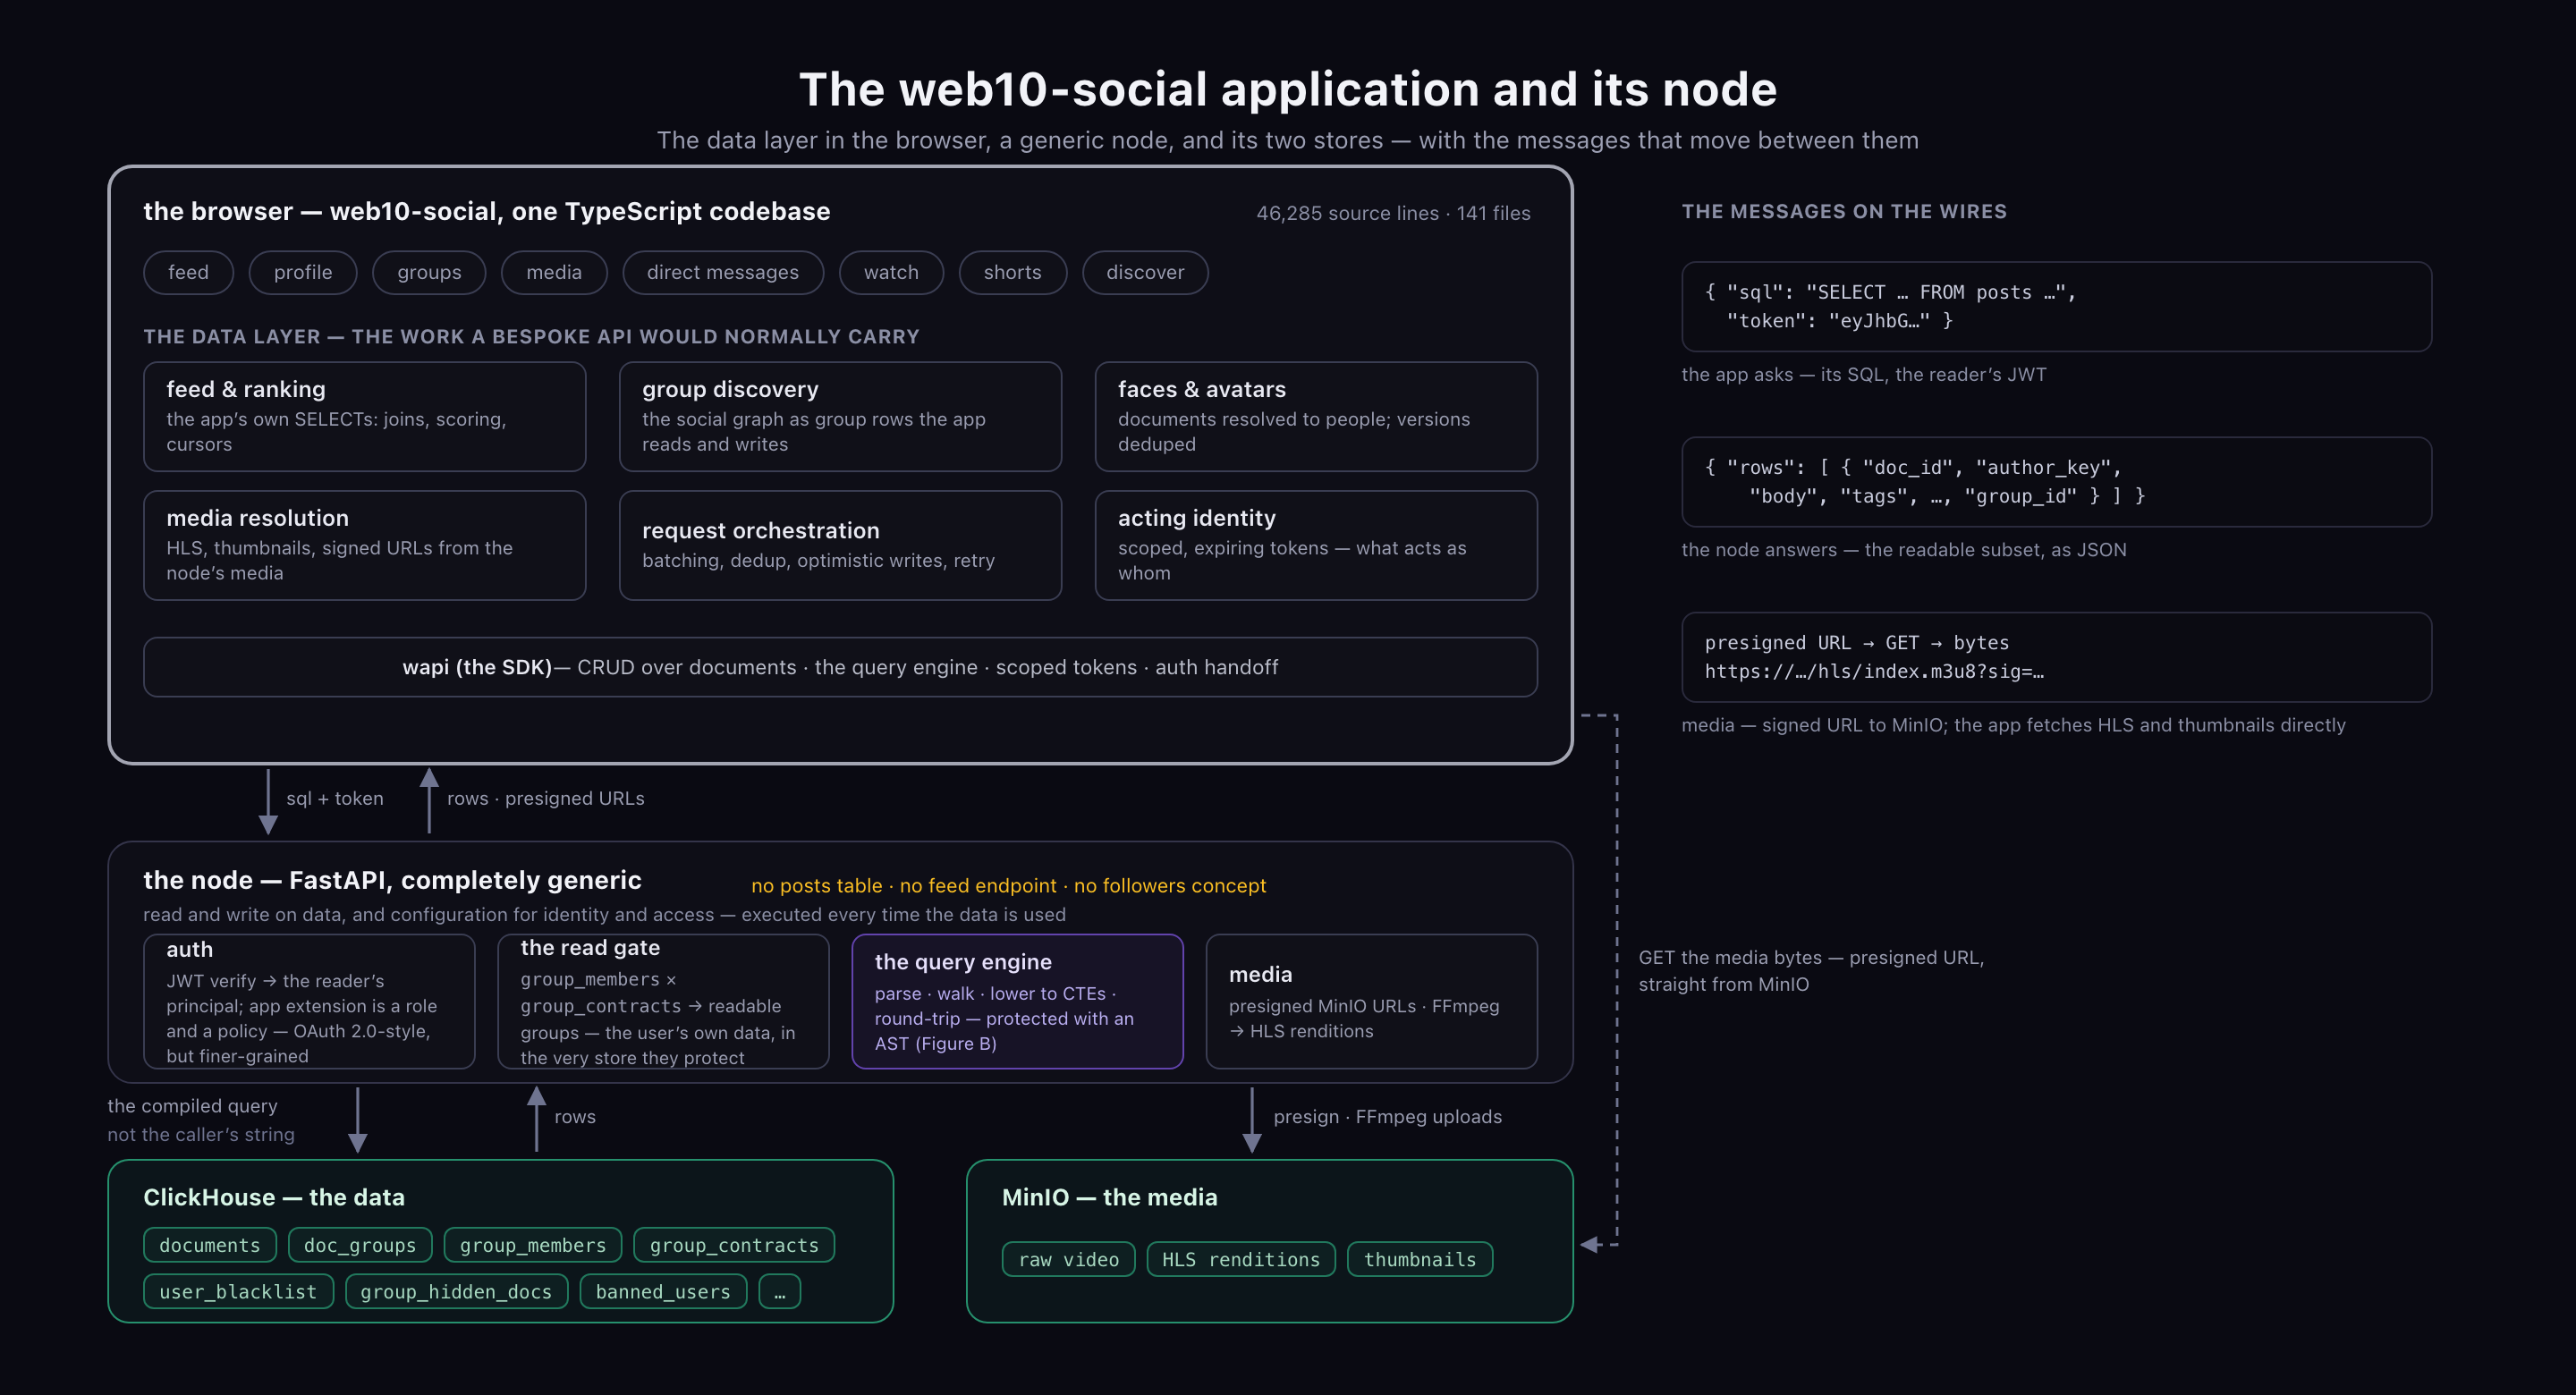
\includegraphics[width=\textwidth]{figs/fig-app-arch.png}
  \caption{The web10-social application and its node---the data layer in the
  browser, a generic node, and its two stores, with the messages that move
  between them. The browser frame holds the application's surfaces and the
  six data-layer modules a bespoke API would normally carry: feed and
  ranking (the app's own queries: joins, scoring, cursors), group discovery
  (the social graph as group rows the app reads and writes), faces and
  avatars, media resolution, request orchestration (batching, dedup,
  optimistic writes, retry), and acting identity (scoped, expiring tokens---
  what acts as whom)---plus the SDK. The node frame is thin and generic:
  authentication, the read gate, the query engine, and media (signed URLs
  to object storage; the render pipeline to HLS renditions). The stores are
  drawn with their real names: ClickHouse's \texttt{documents} and group
  tables, and the object store's media keys. The messages panel shows the
  payloads that move: \texttt{sql + token} down; the compiled query---not
  the caller's string---and rows with signed URLs back; then the signed URL,
  the GET, and the bytes. Pinned: 46,285 lines of application-local source
  across 141 files (\S\ref{sec:extend}).}
  \label{fig:app-arch}
\end{figure*}

%=============================================================================
\section{The node stays generic; the rules are your data}
\label{sec:access}

The node that hosts web10 knows one thing, and it is not a social
concept. It gives an application read and write on the data, and it
gives it configuration for identity and access---and it executes that
configuration every time the data is used. The platform API has no
\texttt{posts} table, no feed endpoint, no followers construct: the
harder the killer app pushes for bespoke surface (\S\ref{sec:lessons}),
the harder the node resists, because the next application---a notes app,
a music app, a shop---defines identity differently or has no followers
concept at all. The test that keeps the line: \emph{would a notes app, a
music app, or a shop use this endpoint?} Four such surfaces were built
and removed from this node; the list is in \S\ref{sec:lessons}.

What the node is not generic about is the access model---because the
access model belongs to the user. A grant is a \emph{row}: a principal,
a group, and a role, where a role is a per-service permission map---a
bundle named by the application that says \texttt{posts: readAll,
create, updateOwn} and \texttt{comments: readAll}. Two rows carry the
classes \texttt{anyone} and \texttt{authenticated}; a public group is a
group that holds an \texttt{anyone} reader row. There is no visibility
column, because publicness \emph{is} a grant: ``make my group public''
is the act of writing that row, and ``private'' is the absence of it.
One mechanism, and it composes---a group can be invite-only to
\emph{join} and still publicly \emph{readable}, which is exactly the
discovery board.

The operations this model exposes are the operations a cloud operator
would express as policies---principal, service, operation, grant---but
the user who expresses them is the end user, over their own data. The
user revokes an app without leaving a group, leaves a group without
touching an app grant, and rewrites their own publicness the way the
platform's IAM owner would: as data, in the store, through the same API
the applications use. A revoked grant is a tombstone; the checks that
follow read the latest row.

That last sentence is the whole argument's forcing move. Because a
grant is a row, the set of groups a reader may see---their readable
set---is computable \emph{before} any query runs, from data the user
owns, in the same store the query will touch. A wall can be built on
that; a filter cannot. \S\ref{sec:boundary} builds it.

Media moves the same way it is checked: structured documents reference
objects in the node's object storage, and the node issues short-lived
presigned URLs---and, for video, signed HLS manifests and segment
capabilities---after the document's own access check, so the bytes have
the document's authority and its expiry.

%=============================================================================
\section{One store at the bottom: ClickHouse, and the fork Solid did not
take}
\label{sec:store}

At the bottom of the system is ClickHouse~\cite{clickhouse2024}---an
open-source columnar engine built for real-time analytics over
billions of rows, in a way that scales. The platform's answer to
``where does a user's data live?'' is deliberately unglamorous: on each
node, the user's content and the platform's access metadata live in
\emph{one} columnar database. The user namespace is logical isolation
within that table---not a per-user database, not a physical
collection; updates insert a newer version, deletes insert tombstones,
and reads select the latest row and only then drop the deleted ones.

The multi-tenant literature places its tenants at the
\emph{organization}: shared tables carrying an organization
identifier~\cite{force2009}, schema-mapping
techniques~\cite{aulbach2008}, and the shared-versus-separate
spectrum~\cite{jacobs2007}. web10 takes the
spectrum to its limit: one logical tenant per \emph{end user}, in a
shared columnar store. Physical isolation was never what the access
model needed. The isolation a reader requires---``show me only what I
may see''---is a property of the \emph{query}, and
\S\ref{sec:boundary} supplies it at the query boundary.

web10 deliberately trusts the node operator with readable content:
search, ranking, moderation, and audit operate on plaintext; the node
is readable by design, and operator-blindness is not a goal. The stance
is the opposite of the familiar decentralization bet, and it is worth
stating plainly because the nearest prior work takes it.
Solid~\cite{solid2016} keeps its data encrypted and pod-bound for
ownership. web10 makes the opposite bet: the data sits unencrypted and
readable on the node, because that is what makes the high-performance
ClickHouse queries and the data-lakehouse composition of this section
possible---and the bet is that users do not care that the node operator
can read their data, because they own the control over who \emph{else}
can reach it: a grant the user gives is a row the user deletes, and the
operator is bound by law, not encryption, not to tamper with it. What
the user owns is the policy, not the secrecy. End-to-end private
messaging already exists (Signal, WhatsApp); web10 does not compete
with it, and it is not trying to.

The consequence of the readable, shared store is the fork
Figure~\ref{fig:composition} draws. A web10 node pools millions of
users in one shared store, so discover, trending, and ranking are just
queries the application writes against it---cross-author relational
composition inside a single analytical engine, with no cross-database
synchronization dependency. Solid cannot take that fork: each user's
data lives in that user's own pod, so a cross-user query must pull the
whole network, and it does not terminate at scale. ``Who is trending?''
is not a query Solid can run; it is a crawl. The costs of the shared
table are real, and they are the day-to-day operating envelope of
\S\ref{sec:lessons}: version deduplication on every read, merge
pressure, point queries paid to an engine built for scans, and shared
resources between tenants.

\begin{figure*}[t]
  \centering
  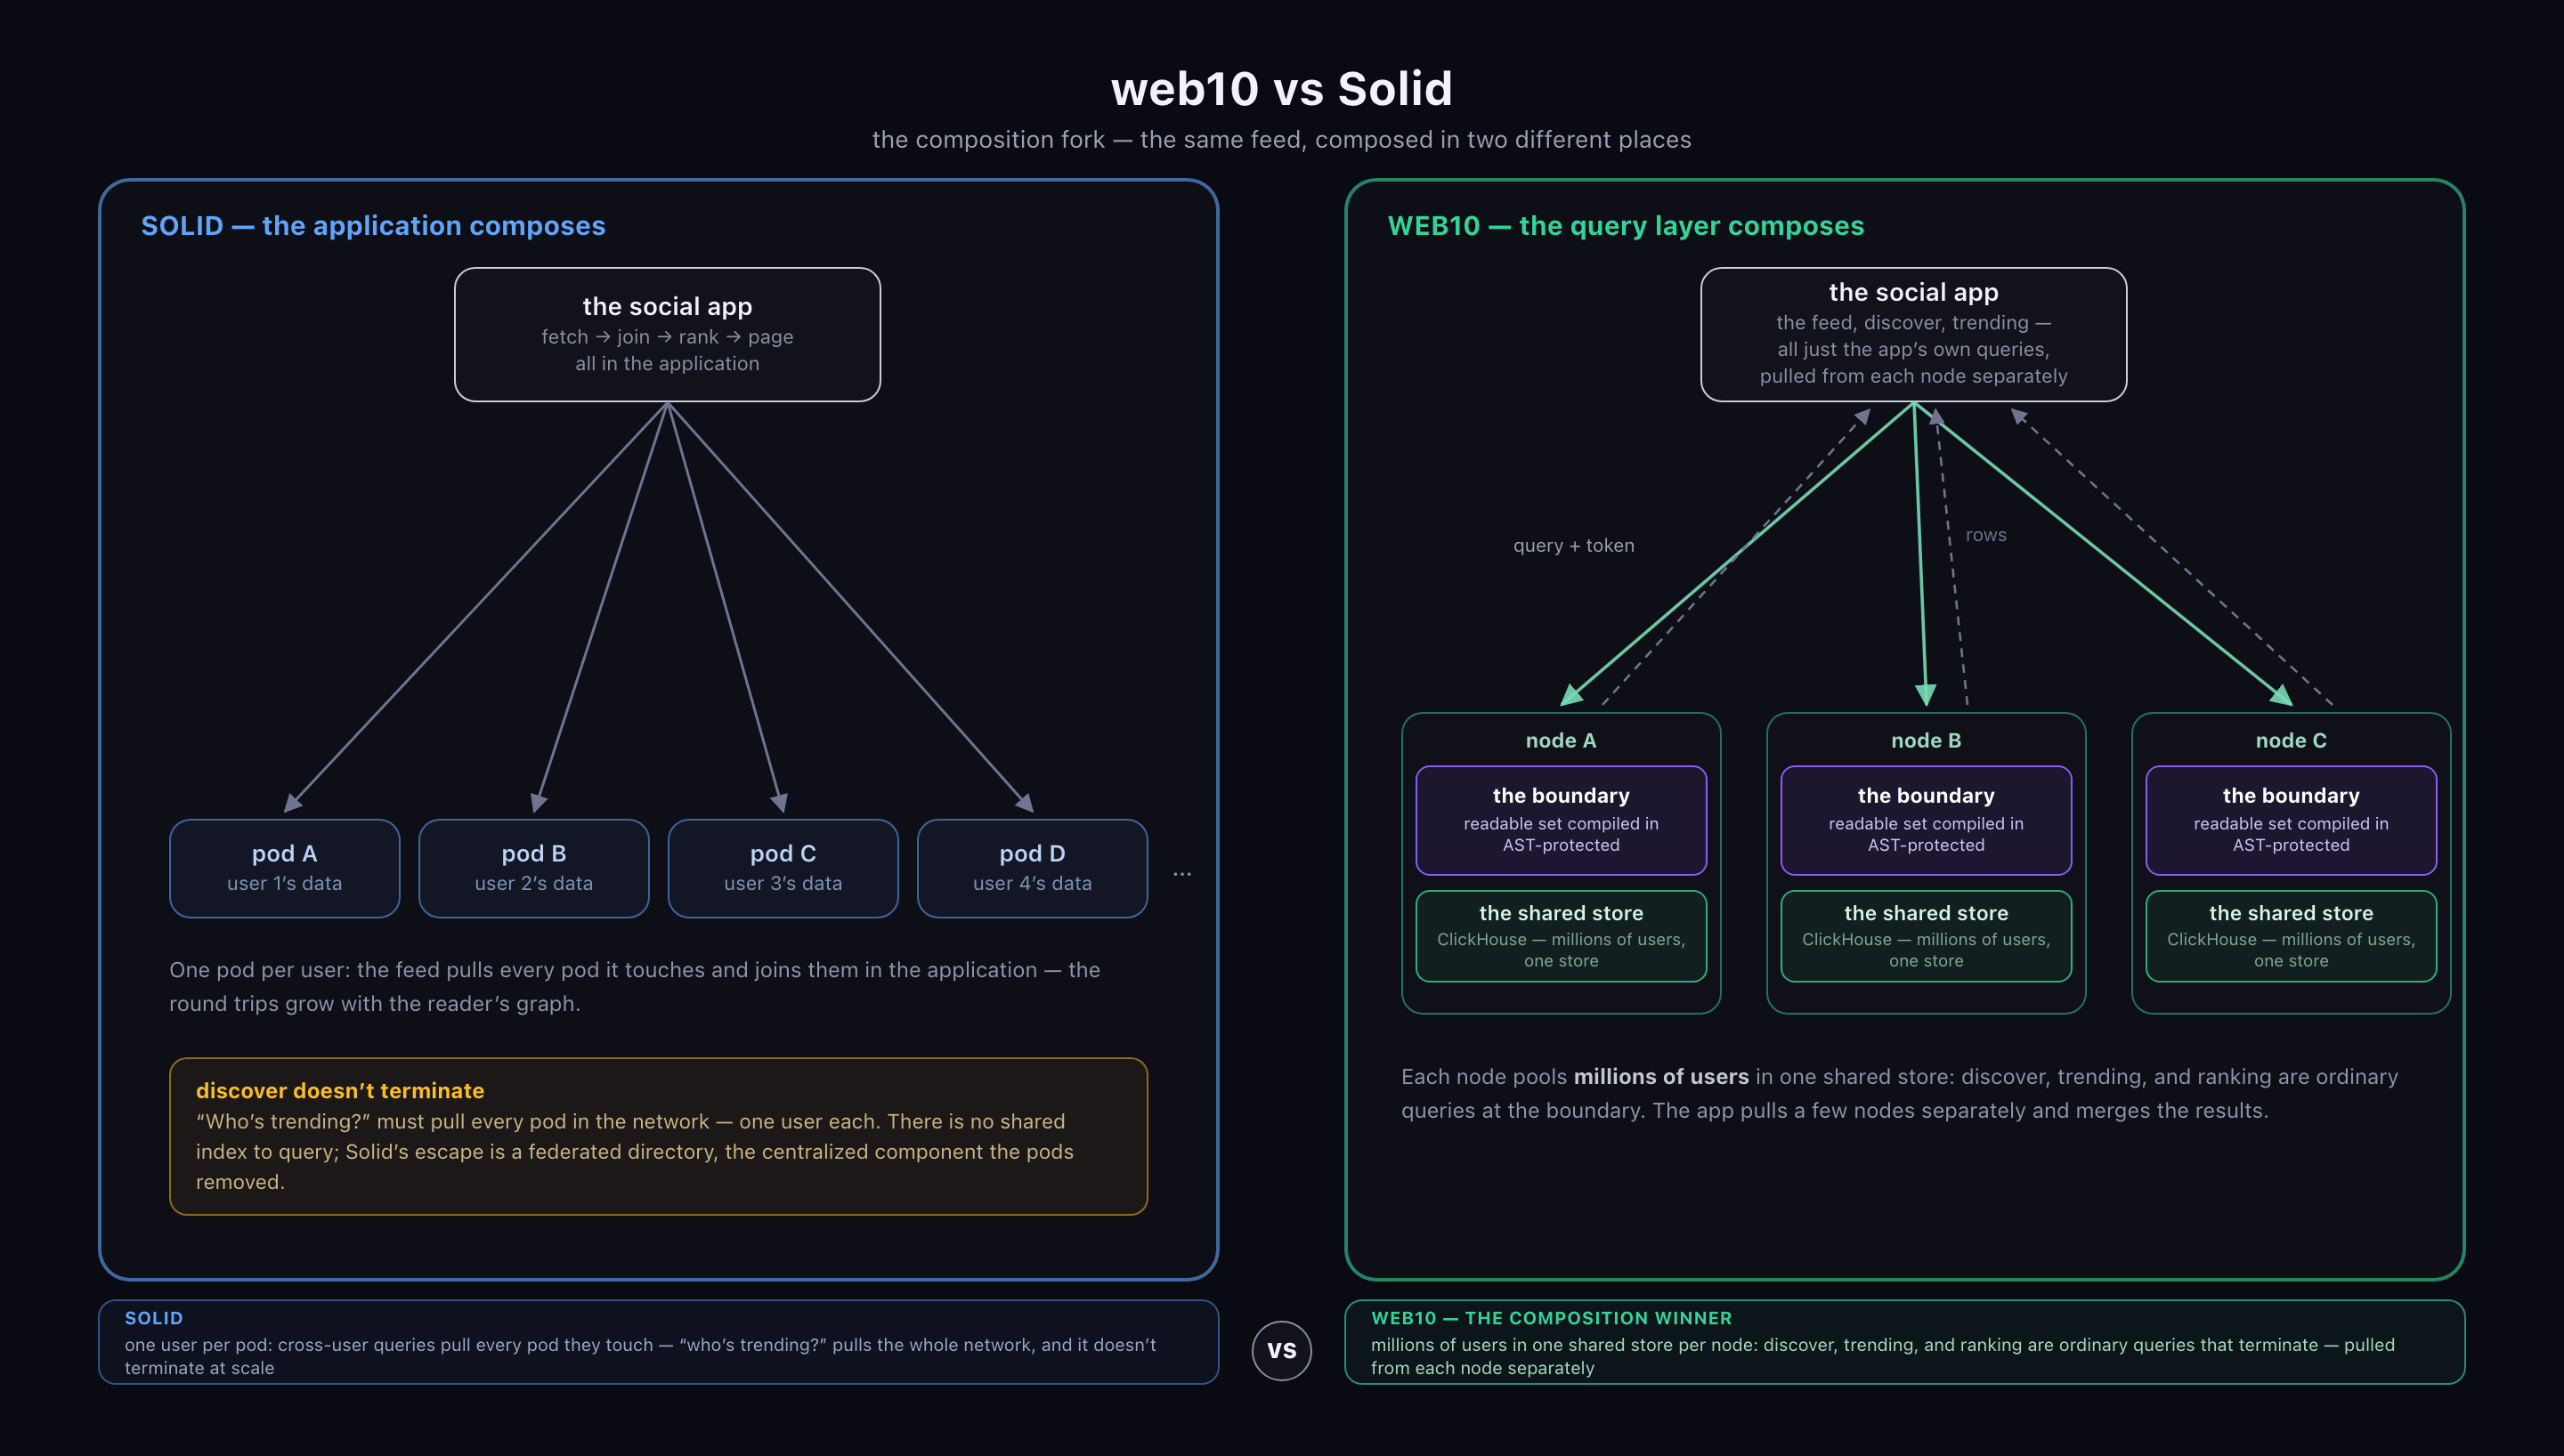
\includegraphics[width=\textwidth]{figs/fig-composition.png}
  \caption{web10 vs Solid: where the composition happens---the same feed,
  composed in two different places. Left: Solid's one-user-per-pod store: a
  cross-user read pulls every pod the query touches, and a discover-type
  query must pull the whole network, so it does not terminate at scale.
  Right: three web10 nodes, each pooling millions of users in one shared
  ClickHouse store; discover, trending, and ranking are ordinary queries the
  application writes against it, each node re-checking the reader's rules on
  every read. The strip names the win: composition---a cross-user query that
  terminates (\S\ref{sec:boundary}, \S\ref{sec:positioning}).}
  \label{fig:composition}
\end{figure*}

%=============================================================================
\section{The boundary: your query, compiled before it runs}
\label{sec:boundary}

Application-written SQL over a multi-tenant store needs a decision
before the caller's relational operations run. The division of labor is
the point: the application's developer writes the query and tunes it;
the platform guarantees the boundary, not the performance. The API
accepts a constrained read-only SQL surface---not arbitrary database
access---and its boundary is a \emph{wall, not a membrane}.

The natural design is a membrane: wrap the caller's query and filter
the \emph{result}. It fails for one reason, and the reason is the whole
section---the caller's query has already read the raw table inside the
parentheses, and an outer filter cannot undo an aggregation that baked
everyone's data in:

\begin{lstlisting}[style=sql]
-- counts every user's comments; the outer group filter is too late
SELECT author_key, count(*)
FROM documents WHERE collection_name = 'comments'
GROUP BY author_key
\end{lstlisting}

The aggregate has collapsed all authors into counts before any
row-level filter could run. Filtering the output of an aggregation is
not access control.

web10 redirects the input instead. The node parses the caller's SQL to
an AST and never sends that original string to the engine: it walks
every table reference, rejects the raw node tables, the table
functions, and the services the reader is not granted, and lowers each
granted service name to a \emph{boundary CTE}---the service's documents
deduped to the latest not-deleted row, joined to the current
\texttt{doc\_groups} mappings, filtered to the reader's readable groups
inlined from the read gate, with the block, sharing, hidden-document,
and node-ban exclusions applied. The readable set of
\S\ref{sec:access} is materialized \emph{before} the caller's joins and
aggregation run; an empty set yields an empty service. The query that
executes is emitted from the validated AST, re-parsed on the way out and
required to come back as exactly one statement---the caller's string is
never executed, and Figure~\ref{fig:query-engine} follows one feed
query through all of it.

The OLTP-era answer to many users on one database was row-level
security inside the engine: PostgreSQL's row-security
policies~\cite{postgres-rls} evaluate a per-row policy expression while
the engine runs the query. On a columnar store the boundary moves to
the query, where the readable set is compiled in before any data moves.
Both placements are sound; the cost of each is the matched workload
\S\ref{sec:evidence} leaves to run.

\begin{figure*}[t]
  \centering
  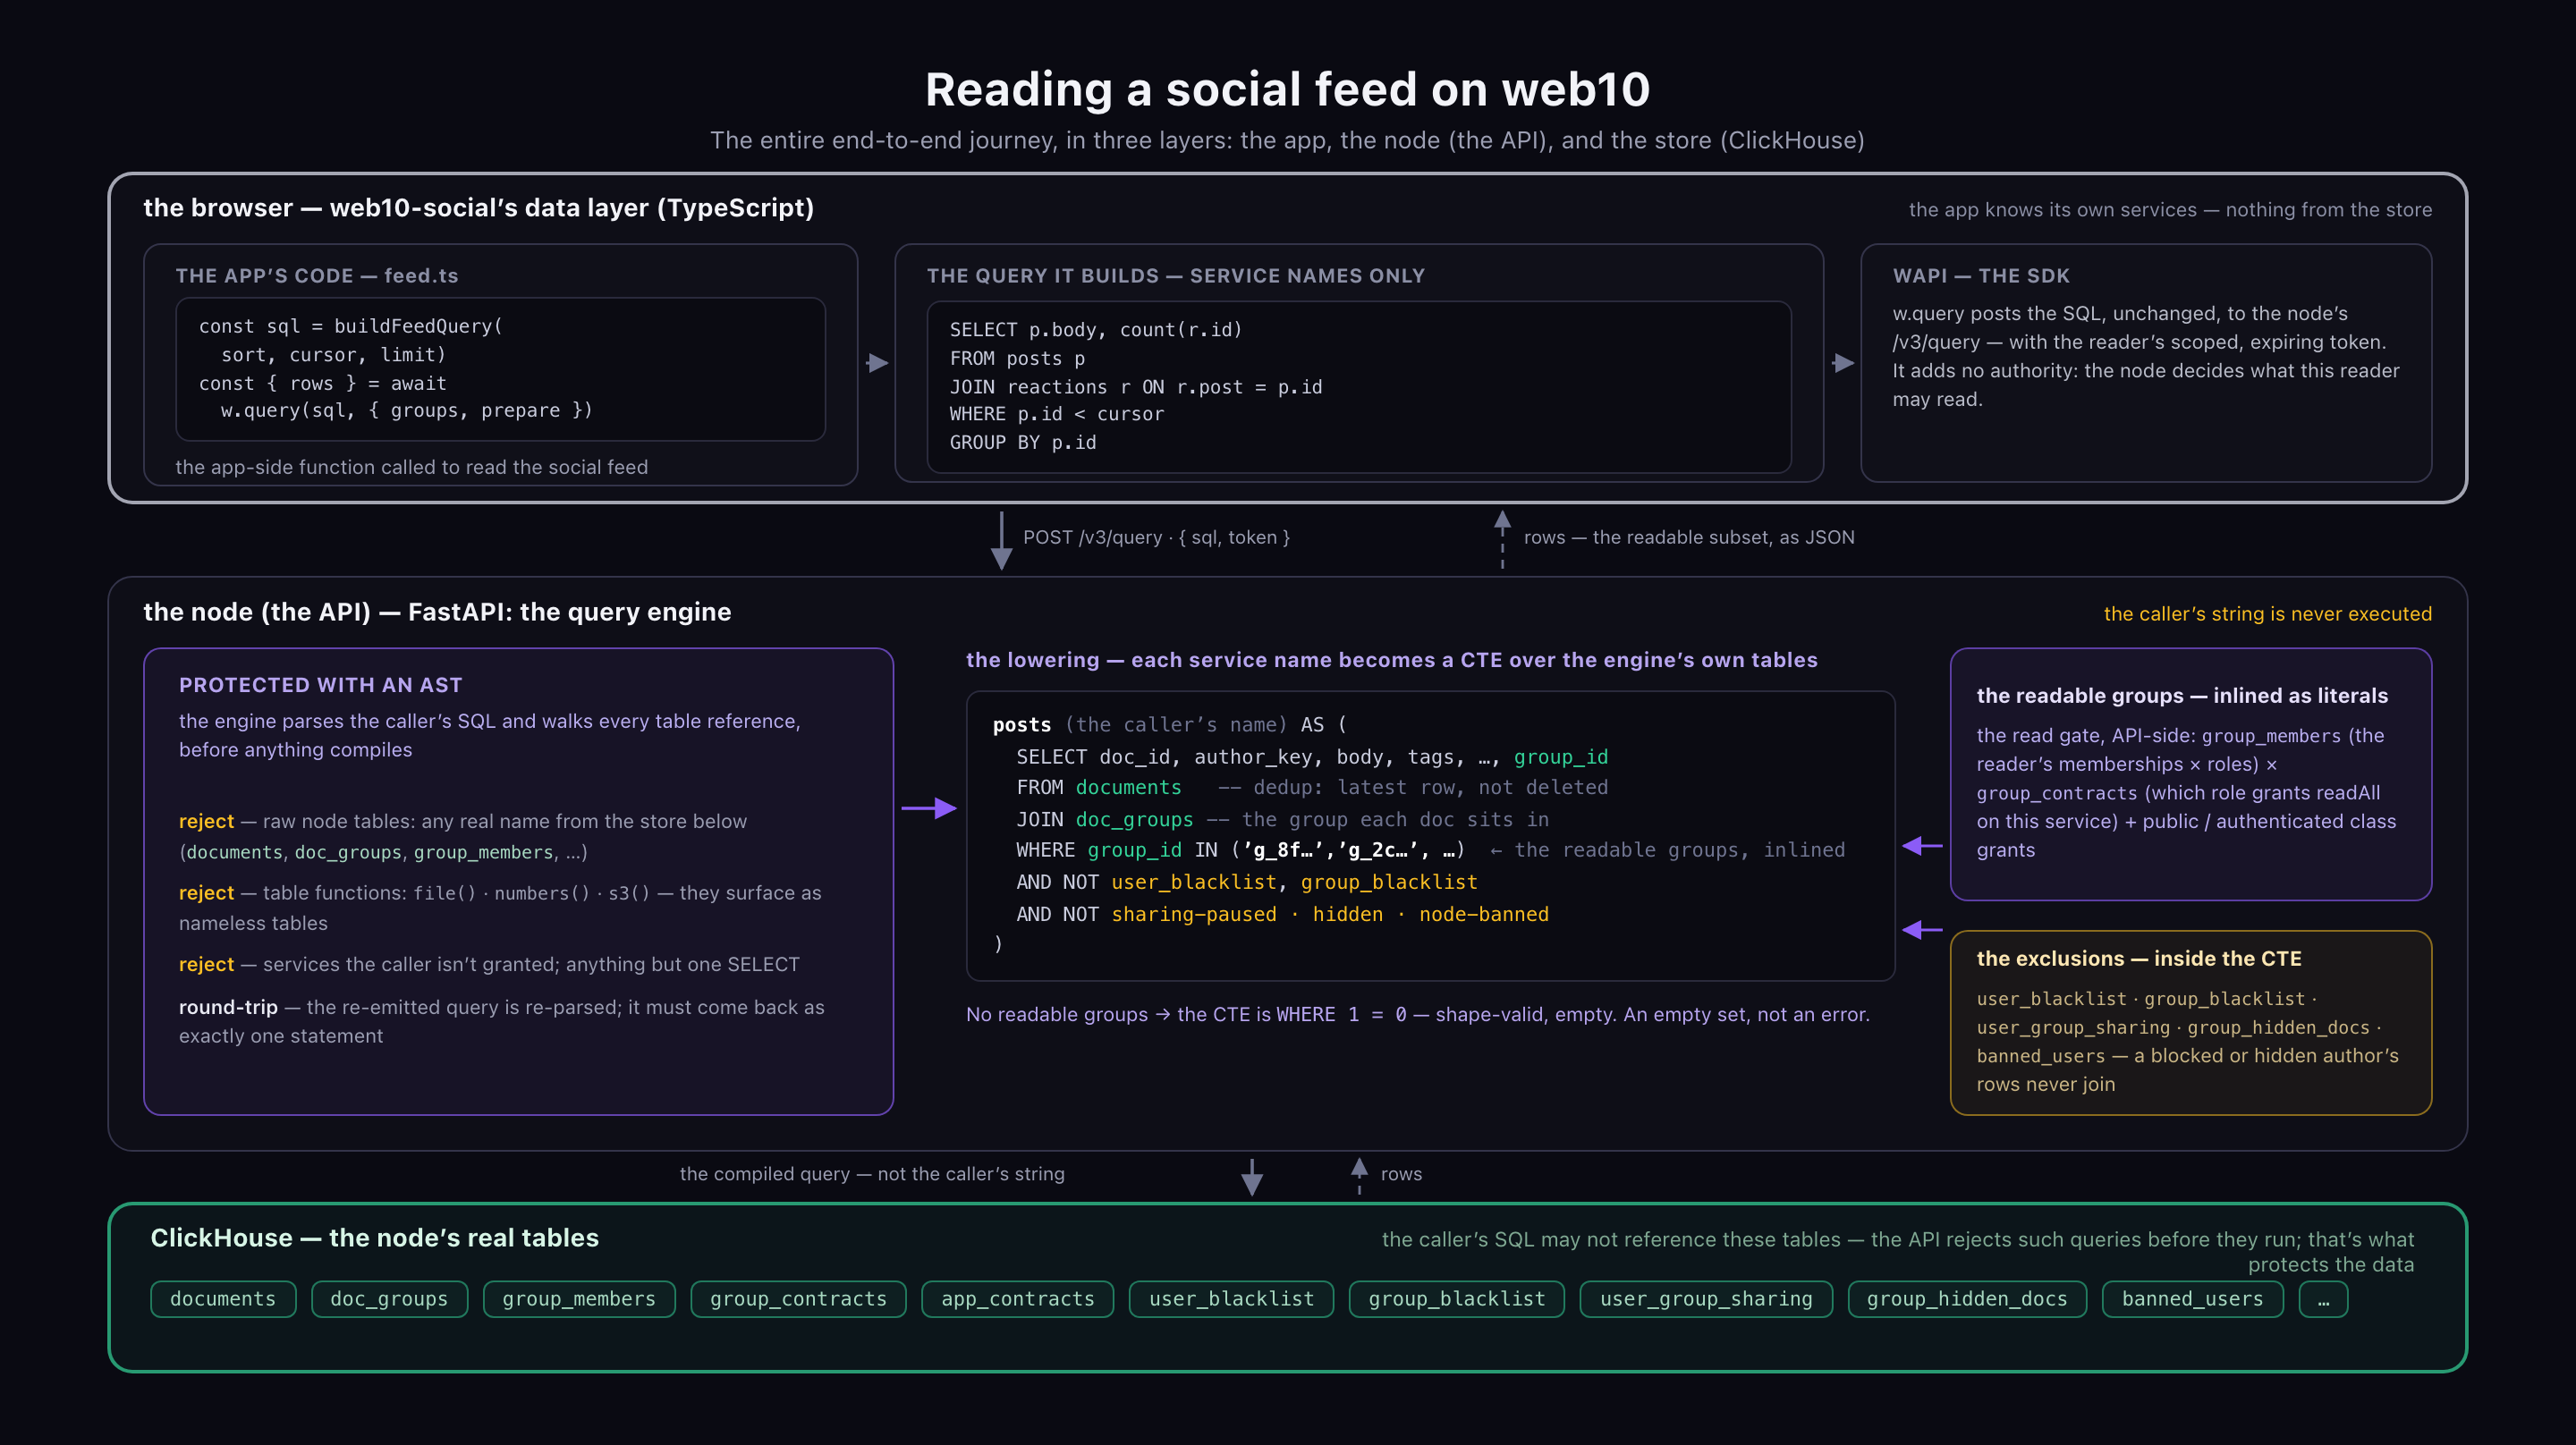
\includegraphics[width=\textwidth]{figs/fig-query-engine.png}
  \caption{Reading a social feed on web10: the entire end-to-end journey, in
  three layers---the app, the node (the API), and the store (ClickHouse).
  Browser side: the app's feed code builds the query over service names
  (\texttt{posts}, \texttt{reactions}, \texttt{comments},
  \texttt{profile}); the SDK posts \texttt{\{sql, token\}} to
  \texttt{POST /v3/query}---it adds no authority, the node decides what this
  reader may read. Node side: the API parses the SQL to an AST and walks
  every table reference---rejecting raw node tables, table functions, and
  ungranted services, and round-tripping the emitted SQL to exactly one
  statement---then lowers each service name to a boundary CTE over the
  engine's own tables: \texttt{documents} deduped to the latest not-deleted
  row, joined to the current \texttt{doc\_groups} mappings, filtered to the
  reader's readable groups (inlined from the read gate), with the exclusion
  tables applied. The caller's string is never executed: the query that runs
  is emitted from the validated AST, and the ClickHouse strip names every
  real table the caller may not reach.}
  \label{fig:query-engine}
\end{figure*}

%=============================================================================
\section{Extending the platform costs a role and a policy}
\label{sec:extend}

The social application is the node's killer app---the application
compelling enough to pull users onto a new platform---and it is also
the platform's hardest test, because it wants everything a bespoke
backend would have given it. What it got instead is the division of
labor of \S\ref{sec:boundary}: its persistent data and authentication
use the node's document, group, query, and media interfaces; its feeds
are its own queries; its surfaces---text and discussion, image and
mixed-media posts, vertical short video, long-form video, audio---are
services it names over the shared store, composing on the same document,
group, and query substrate rather than shipping a backend per surface.
In the measured source snapshot, the application-local frontend is
\textbf{46,285 physical source lines across 141 files}: 45,846
TypeScript/TSX lines and 439 CSS lines under \texttt{src/}, excluding
tests; counts include comments and blank lines and exclude dependencies
and tooling.
Figure~\ref{fig:groups} shows the social surface the feed composes over:
a group---a shared space on the user's node---whose membership, roles,
and per-post visibility are the application's choices over the generic
grants of \S\ref{sec:access}.

\begin{figure*}[t]
  \centering
  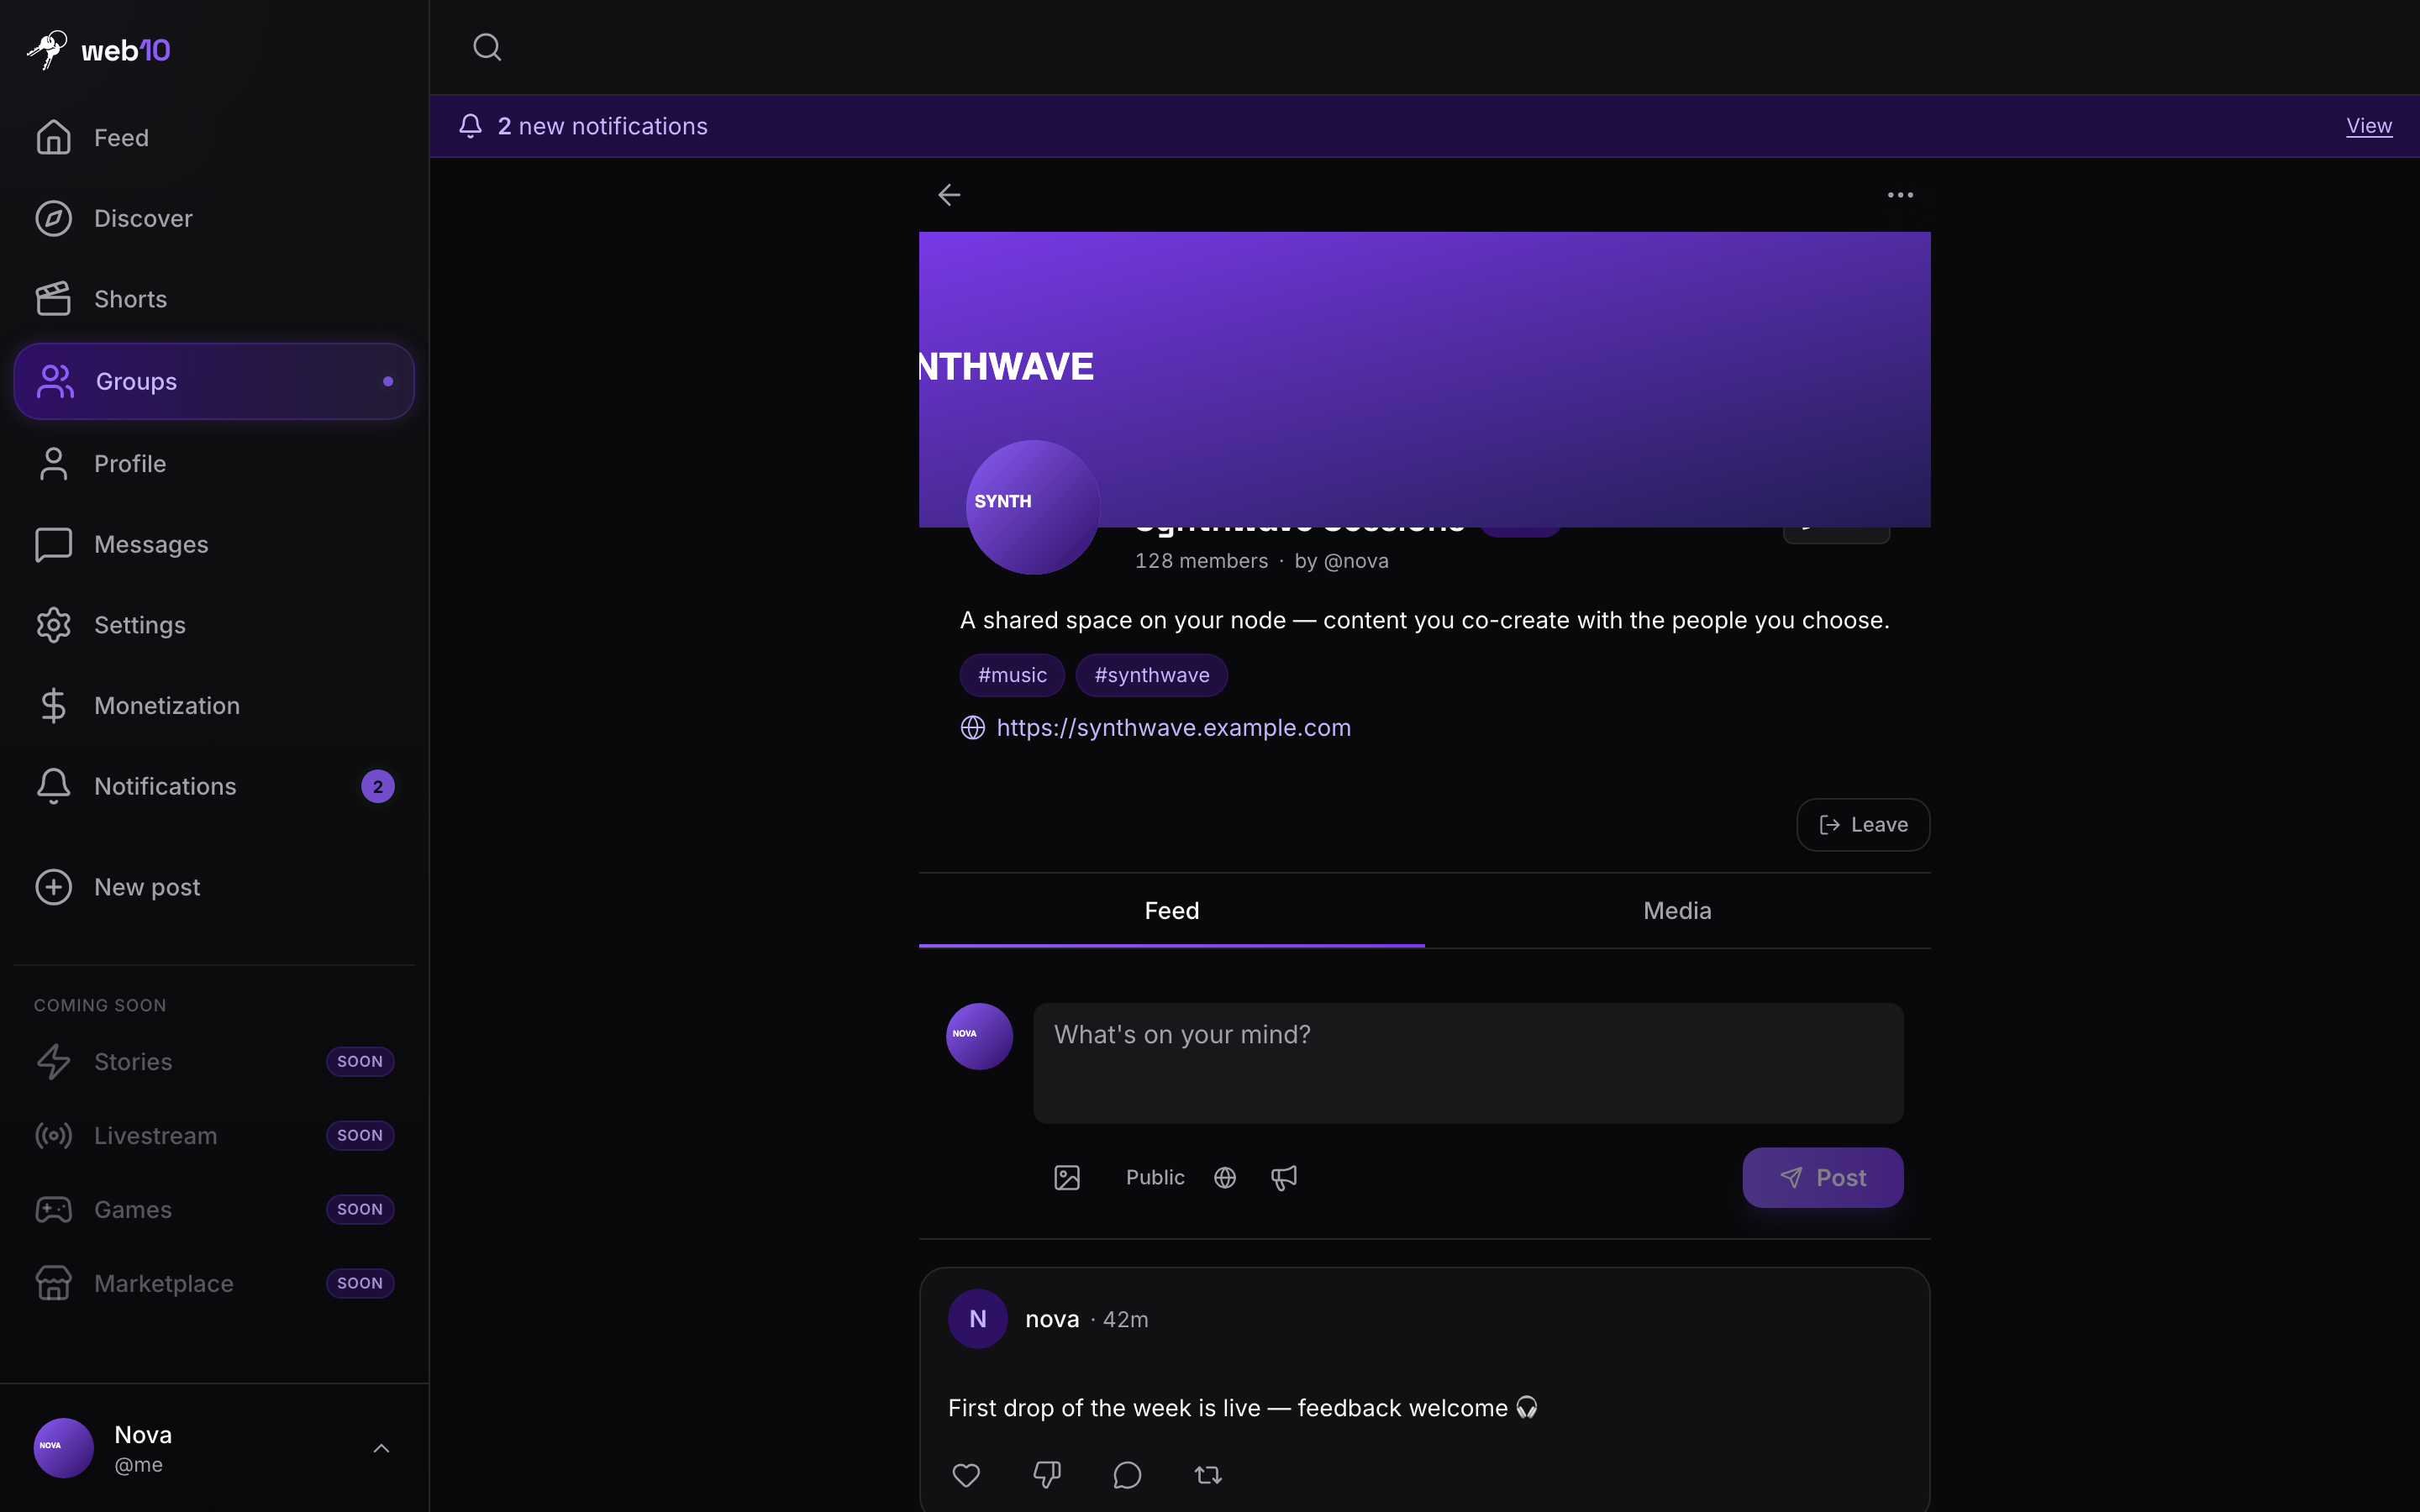
\includegraphics[width=\textwidth]{figs/fig-groups.png}
  \caption{A group---``a shared space on your node.'' Membership, roles, and
  per-post visibility (Public / node / group) expose application choices over
  the generic groups and grants of \S\ref{sec:access}.}
  \label{fig:groups}
\end{figure*}

Extending the platform is as simple as a role and a policy: a new
application gets an app contract, and the user grants it the per-service
reads it needs. It is the same job OAuth 2.0 does for cross-platform
data sharing~\cite{oauth2012}, but the grant names the service, the
group, and the operation---far more fine-grained than a scope. Two
small static applications prove the seam: \emph{Snake} associates
completed runs with player identities; \emph{Marketplace} associates
listings with seller identities. Each writes its own service
(\texttt{snake\_scores}, \texttt{marketplace\_listings}) and reads the
social application's \texttt{profile} documents through the user's own
grants. Neither modified the social application, and neither added a
game, commerce, leaderboard, or seller-profile endpoint to the node.
The common dependency is the document convention and the access
primitives---not an application-specific API agreement:

\begin{lstlisting}[style=sql]
WITH latest_profiles AS (
  SELECT author_key, body FROM profile
  QUALIFY row_number() OVER (
    PARTITION BY author_key
    ORDER BY updated_at DESC, created_at DESC,
             doc_id DESC) = 1
)
SELECT s.author_key,
       JSONExtractInt(s.body, 'score') AS score,
       p.body AS profile_body
FROM snake_scores s LEFT JOIN latest_profiles p
  ON s.author_key = p.author_key
ORDER BY score DESC LIMIT 50
\end{lstlisting}

Both service names resolve to reader-filtered relations before the join,
so permission does not leak through it: an app-level grant on
\texttt{profile} does not itself open a private profile group, and an
ungranted service is rejected before execution. Figure~\ref{fig:interop}
is the result in the browser; Figure~\ref{fig:platforms} is why the
fork matters.

On Mastodon and Bluesky, a second application reads through the
platform's fixed endpoints or replicates the user's records into its own
backend: delegation is app-to-\emph{user}-data, the object model stays
fixed, and there is no shared store to compose across---a new read
pattern is a new backend, and the model has no record shape for a
hi-score or a listing. Here, a second app gets a typed read on the
first app's data and joins it in SQL on one shared columnar store: a
new read pattern is a new query.

\begin{figure*}[t]
  \centering
  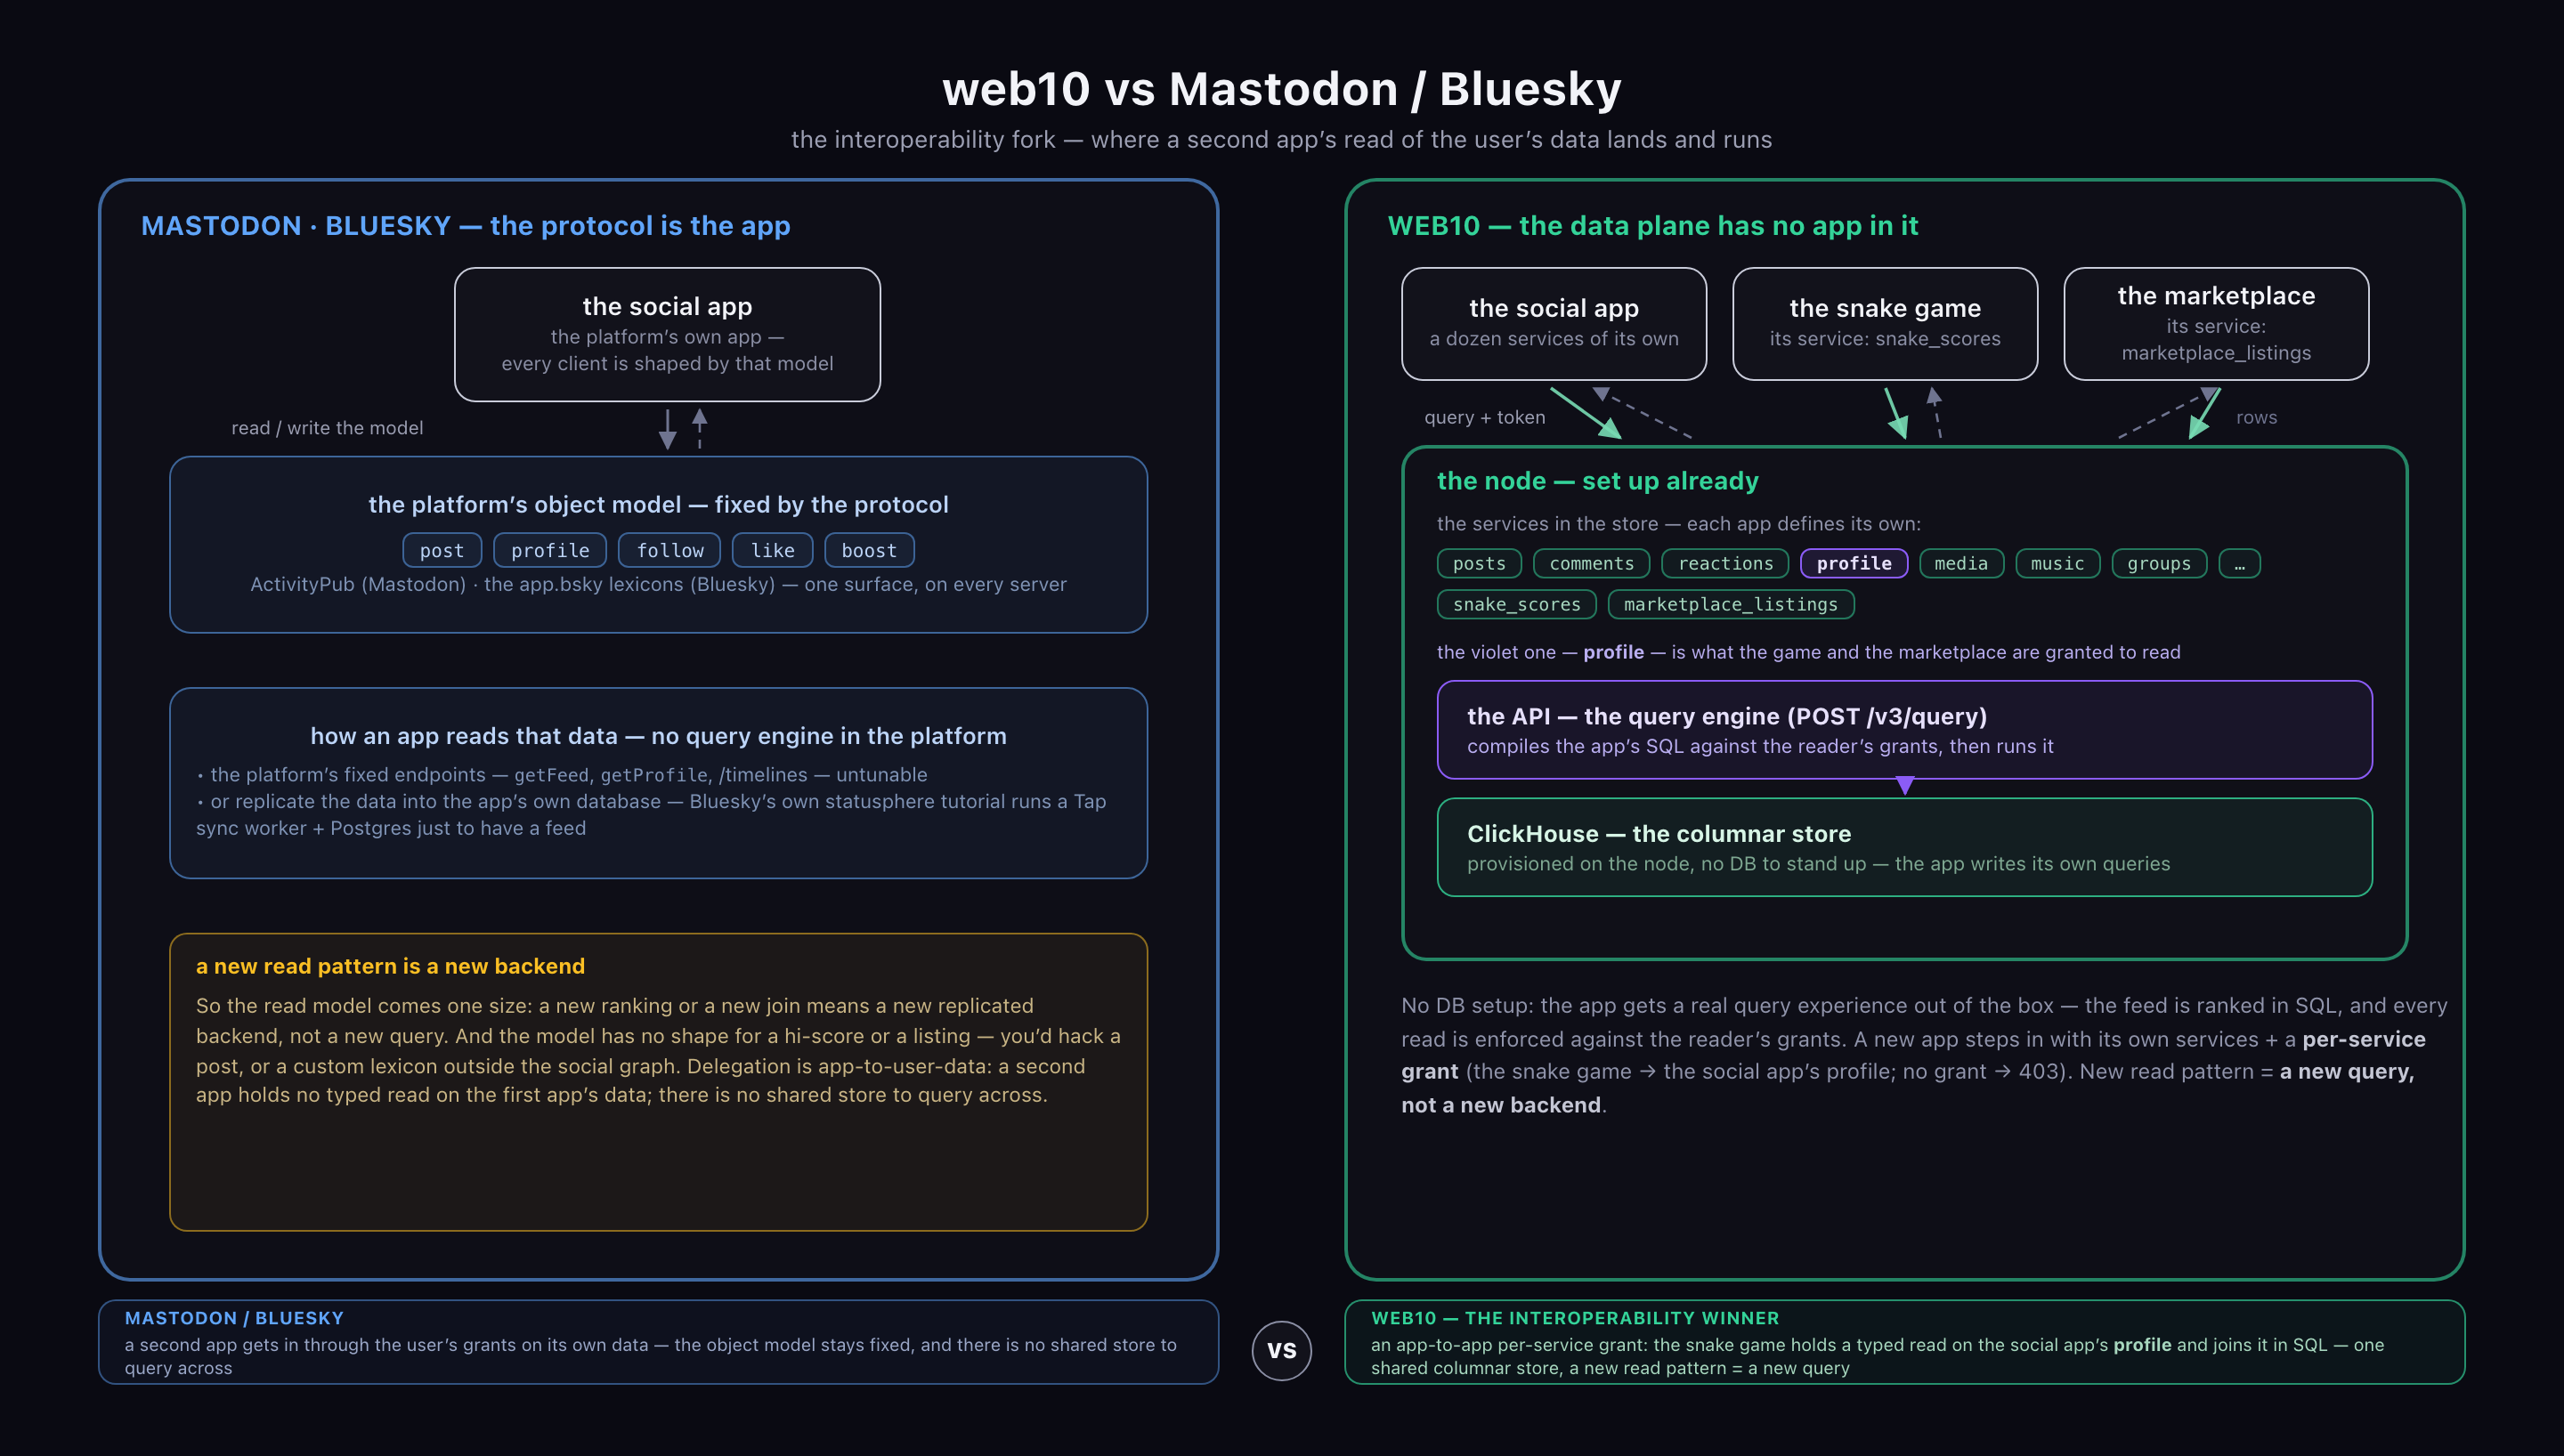
\includegraphics[width=\textwidth]{figs/fig-platforms.png}
  \caption{web10 vs Mastodon / Bluesky: the interoperability fork---where a
  second app's read of the user's data lands and runs. Left: the fixed social
  object model (post $\cdot$ profile $\cdot$ follow $\cdot$ like $\cdot$
  boost); there is no query engine in the platform---the app reads through
  the platform's fixed endpoints (untunable) or replicates records into its
  own database (Bluesky's own statusphere tutorial stands up a sync worker
  and a separate store just to have a feed)---and the model has no record
  shape for a hi-score or a listing. Right: the web10 node, set up already:
  the social app's services (\texttt{posts} $\cdot$ \texttt{comments} $\cdot$
  \texttt{reactions} $\cdot$ \texttt{profile} $\cdot$ \texttt{media} $\cdot$
  \texttt{music} $\cdot$ \texttt{groups} $\cdot$ \ldots; \texttt{profile}
  highlighted---the one the interop grant covers) plus the new apps' own
  (\texttt{snake\_scores} $\cdot$ \texttt{marketplace\_listings}); the API in
  action---the query engine (\texttt{POST /v3/query}) compiles the app's
  query against the reader's grants, then runs it---over the ClickHouse
  columnar store, provisioned on the node, no database to stand up; a second
  app steps in through a per-service grant the user gives, and no grant, no
  read. The strip scores the matchup: web10---the interoperability winner
  (an app-to-app per-service grant on one shared columnar store; a new read
  pattern is a new query, not a new backend).}
  \label{fig:platforms}
\end{figure*}

\begin{figure*}[t]
  \centering
  \begin{minipage}[t]{0.46\textwidth}
    \centering
    \textbf{Snake: earned score + social identity}\\[4pt]
    
\includegraphics[width=\linewidth]{../interoperability-demo/figures/snake-identity.png}
  \end{minipage}\hfill
  \begin{minipage}[t]{0.46\textwidth}
    \centering
    \textbf{Marketplace: listing + social identity}\\[4pt]
    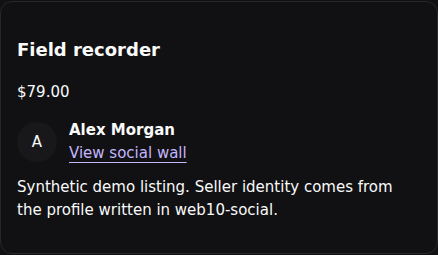
\includegraphics[width=\linewidth]{../interoperability-demo/figures/marketplace-identity.png}
  \end{minipage}
  \caption{One social-written profile, two application views. Snake joins an
  earned score to the player's profile; Marketplace joins a listing to the
  seller's same profile. These are direct browser element captures, with
  synthetic account and listing data. Full-page, consent, and denial
  captures are retained in the artifact.}
  \label{fig:interop}
\end{figure*}

%=============================================================================
\section{The network: verified, not registered}
\label{sec:network}

The access model of \S\ref{sec:access} is defined for one node. This
section states the model that makes it a network: the address, the
handshake, and the domain.

The identifier is \texttt{provider/username}---the provider is the node,
the username is the user, and the pair is globally unique across the
federation. A user's home node is where their account and their grants
live; a user's following set can span $N$ nodes, and they hold exactly
one account. When that user reads content on another node, they do not
sign up there: their client presents their home-node token, and the
foreign node obtains home-issuer certification, resolves the principal,
and applies its own membership and grant checks. Identity is
\emph{verified, not registered}.

The read model is client-mediated. When the user's feed spans nodes, the
\emph{client} makes the cross-node calls: it holds the home-node token,
groups the following set by provider, and queries only the distinct
nodes the user follows people on---targeted, not broadcast. Each node
returns its own access-gated result set; the client performs the ranked
merge. A node never queries another node's store: the cross-node
boundary is the HTTP API and a verified token, and a foreign node's
response is untrusted content---never query input, never a key into the
local store, never a grant. Database-level cross-server mechanisms
(ClickHouse's \texttt{remote()}/\texttt{cluster()}) are for a trusted
cluster under one operator; using them for federation would make a node
operator's database credentials a federation credential.

\texttt{/certify} is the handshake that makes the verified-not-
registered step cheap. Email has already solved the analogous problem
for messages: an arriving message is asked \emph{is this sender who they
claim to be?} (SPF, DKIM), and that check grants the message no access---
the recipient's own filters still apply. \texttt{/certify} asks the same
of an arriving token: the serving node asks the home issuer, gets one
cached answer per token, and that answer verifies and grants nothing---
a handshake, not a registry, because every node still re-checks its own
rules on every read. Same shape, different mechanism.
Figure~\ref{fig:feed} draws the path for one read: node B authenticates
the home-node token over the issuer's HTTPS \texttt{/certify}, then runs
the same access check node A runs on local reads---contracts and
membership, against B's own store, on every read.

\begin{figure*}[t]
  \centering
  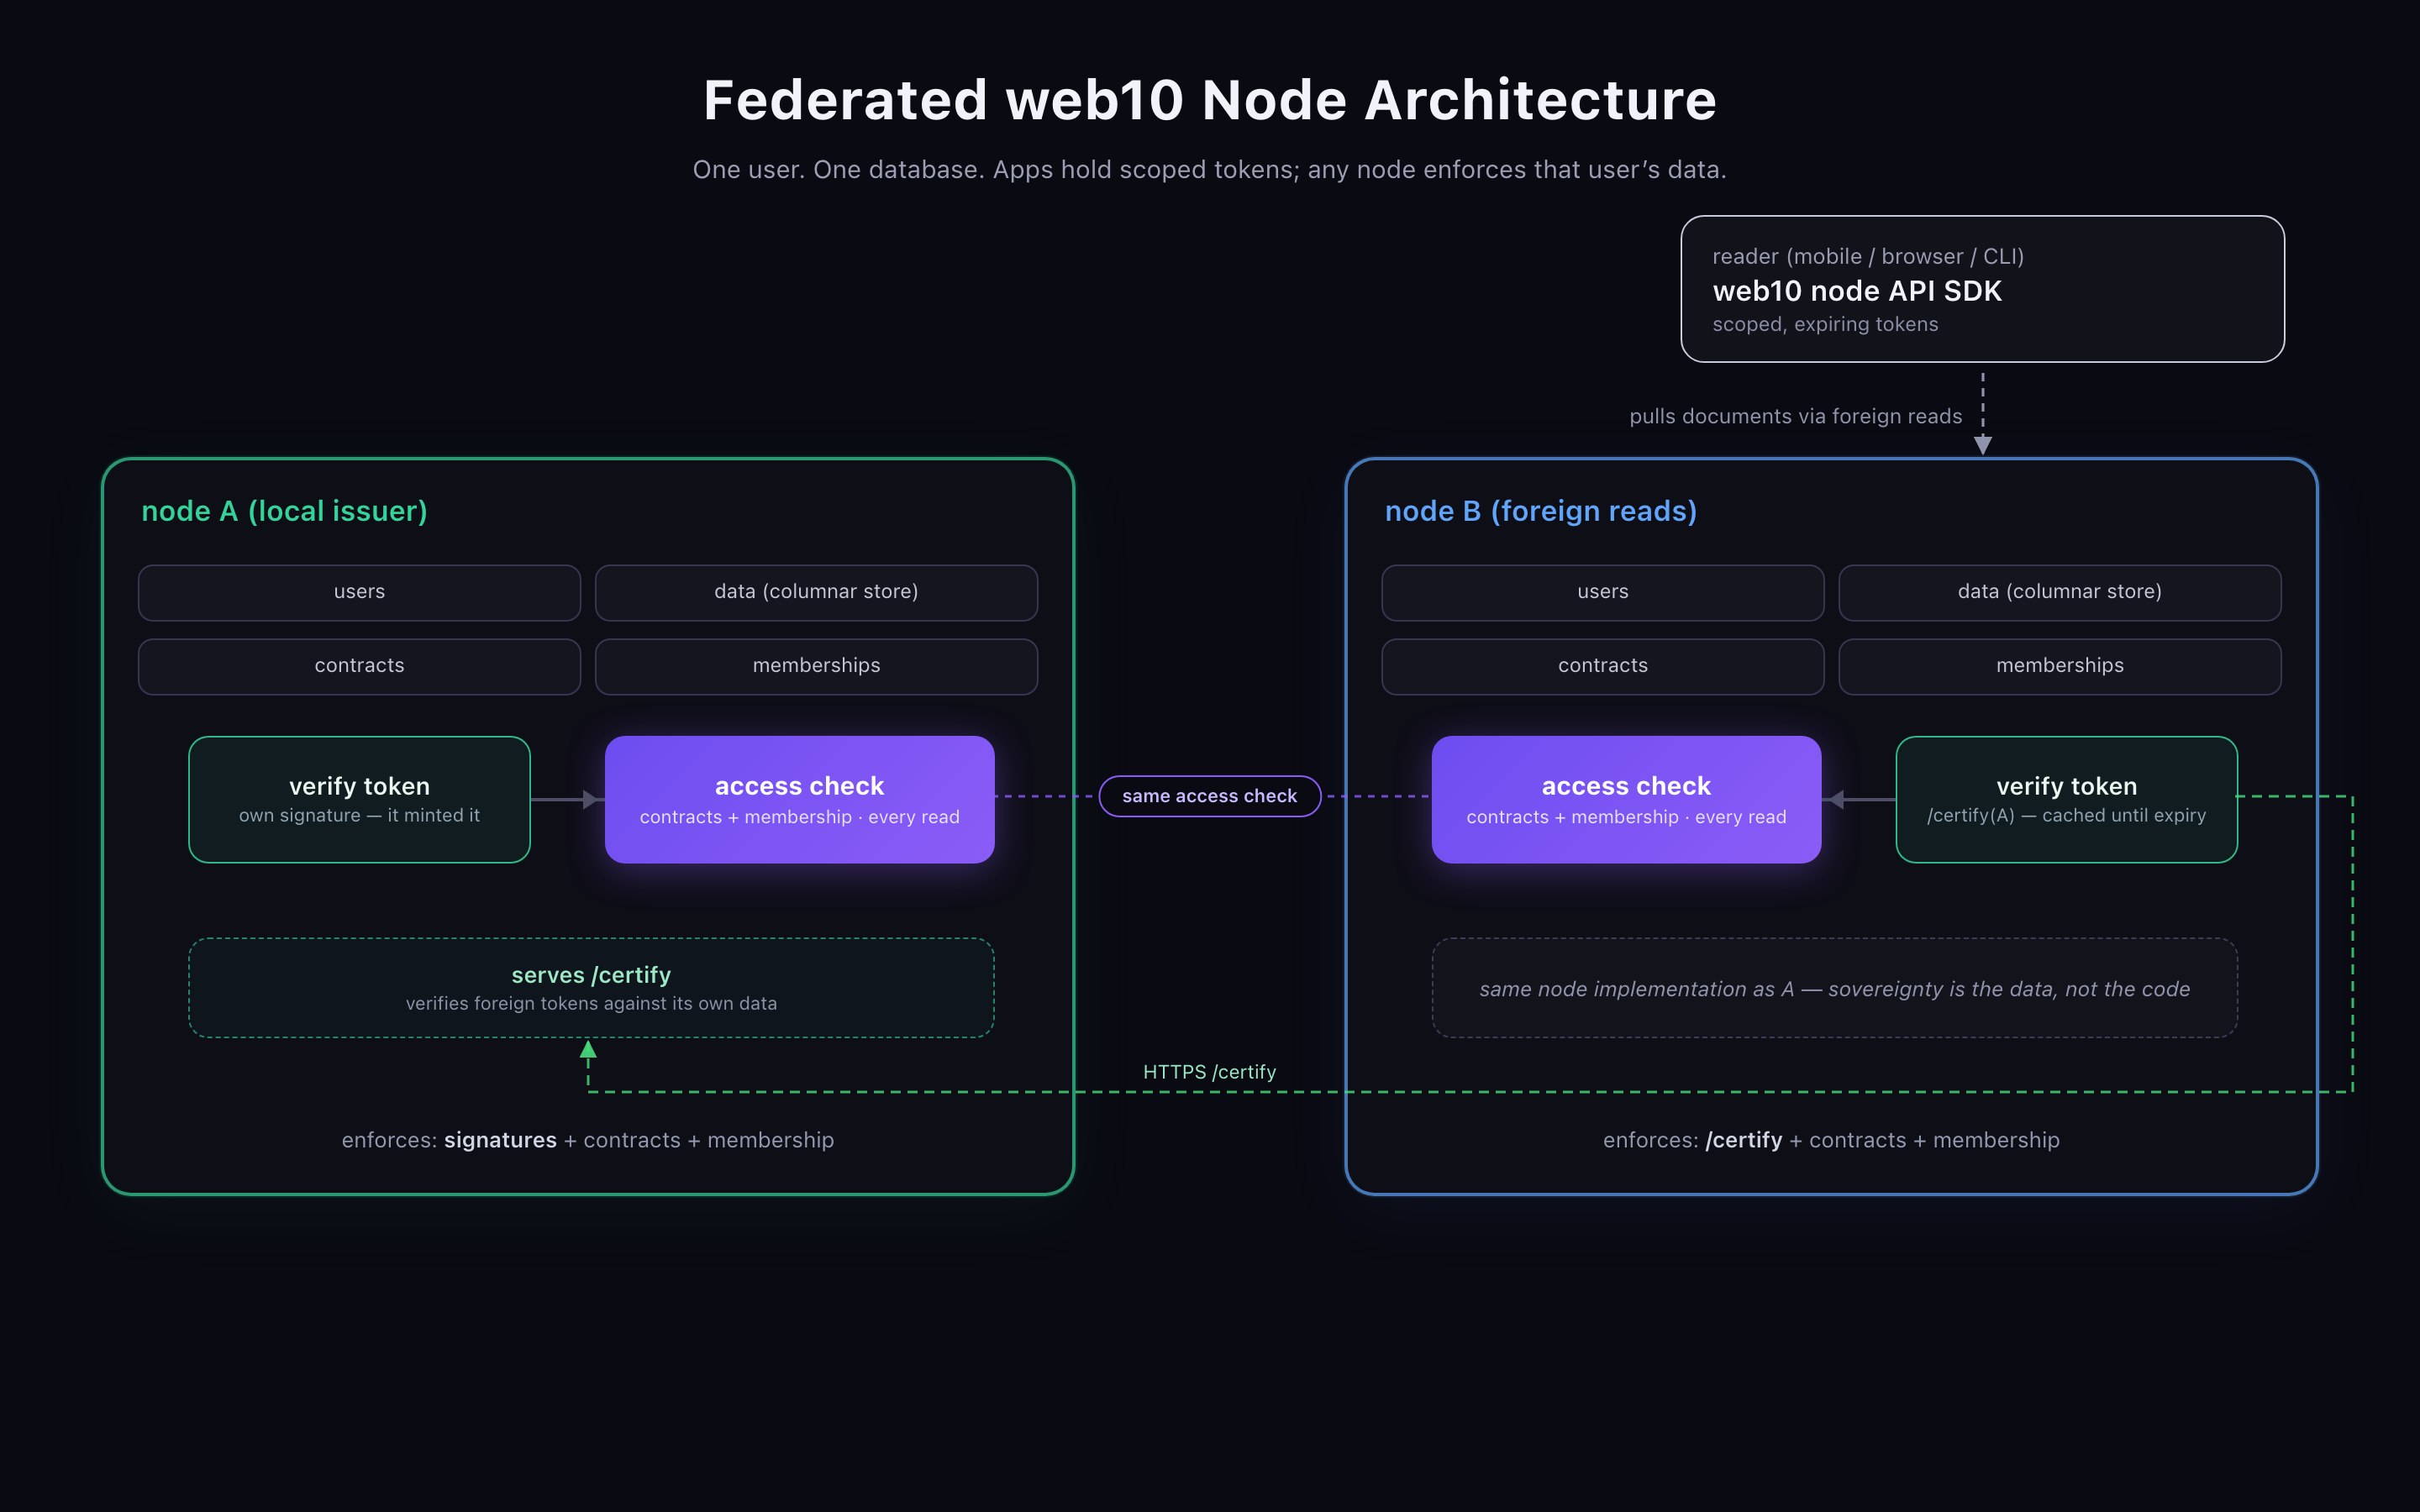
\includegraphics[width=\textwidth]{figs/fig-feed.png}
  \caption{Pulling the web10 feed across nodes. The reader issues reads with
  its home-node token; when a read lands on foreign node B, B authenticates
  the token over the issuer's HTTPS \texttt{/certify}---one cached answer per
  token, never a grant---and then runs the same access check node A runs on
  local reads: contracts and membership against its own store, on every read.
  One node implementation, two sovereign stores; remote data is content,
  never control (\S\ref{sec:network}).}
  \label{fig:feed}
\end{figure*}

The username need not be an opaque string, and this is where the
audience stops belonging to the platform. Through the authenticator's
claim flow, a user binds a DNS domain to their account: a TXT record at
\texttt{web10.\emph{domain}} carries
\texttt{web10.v=1;\allowbreak provider=\emph{node};\allowbreak
user=\emph{username}}, and an authenticated
\texttt{POST /v3/domains/verify} request makes the node perform the DNS
lookup itself, checking that the record names this node and this account
before storing the verified alias. The record is a pointer, not a
credential: DNS lookup is discovery, not authentication, and the
username remains the principal---groups, tokens, and the read gate never
key on the domain. It is the same pattern the web already uses for
identity claims (DKIM, SPF, \texttt{OpenPGPkey}), applied to a social
identity.

The consequence is a \emph{public} subscription that outlives the
provider. The concrete case: a creator's audience follows the domain
\texttt{jacobhoffman.xyz}, not the \texttt{provider/username} the domain
currently points to---which may be one account today and another
tomorrow. The follow is data the \emph{follower} owns: a private
document in the follower's own store whose body is exactly the domain,
written once. When the creator moves---new account, new provider---the
creator re-points the TXT record, and the follows travel with the
domain: the follower's client re-resolves the address on each read, and
no platform holds a ban switch over an address the user keeps. The node
verifies the record by performing the lookup itself, but the record is
untouchable to the node owner, who controls no part of it; a missing or
ambiguous record gives an explicit unavailable state---the follow stays,
and restoring the record recovers it without refollowing.
Figure~\ref{fig:audience-portability} draws the move.

\begin{figure*}[t]
\centering
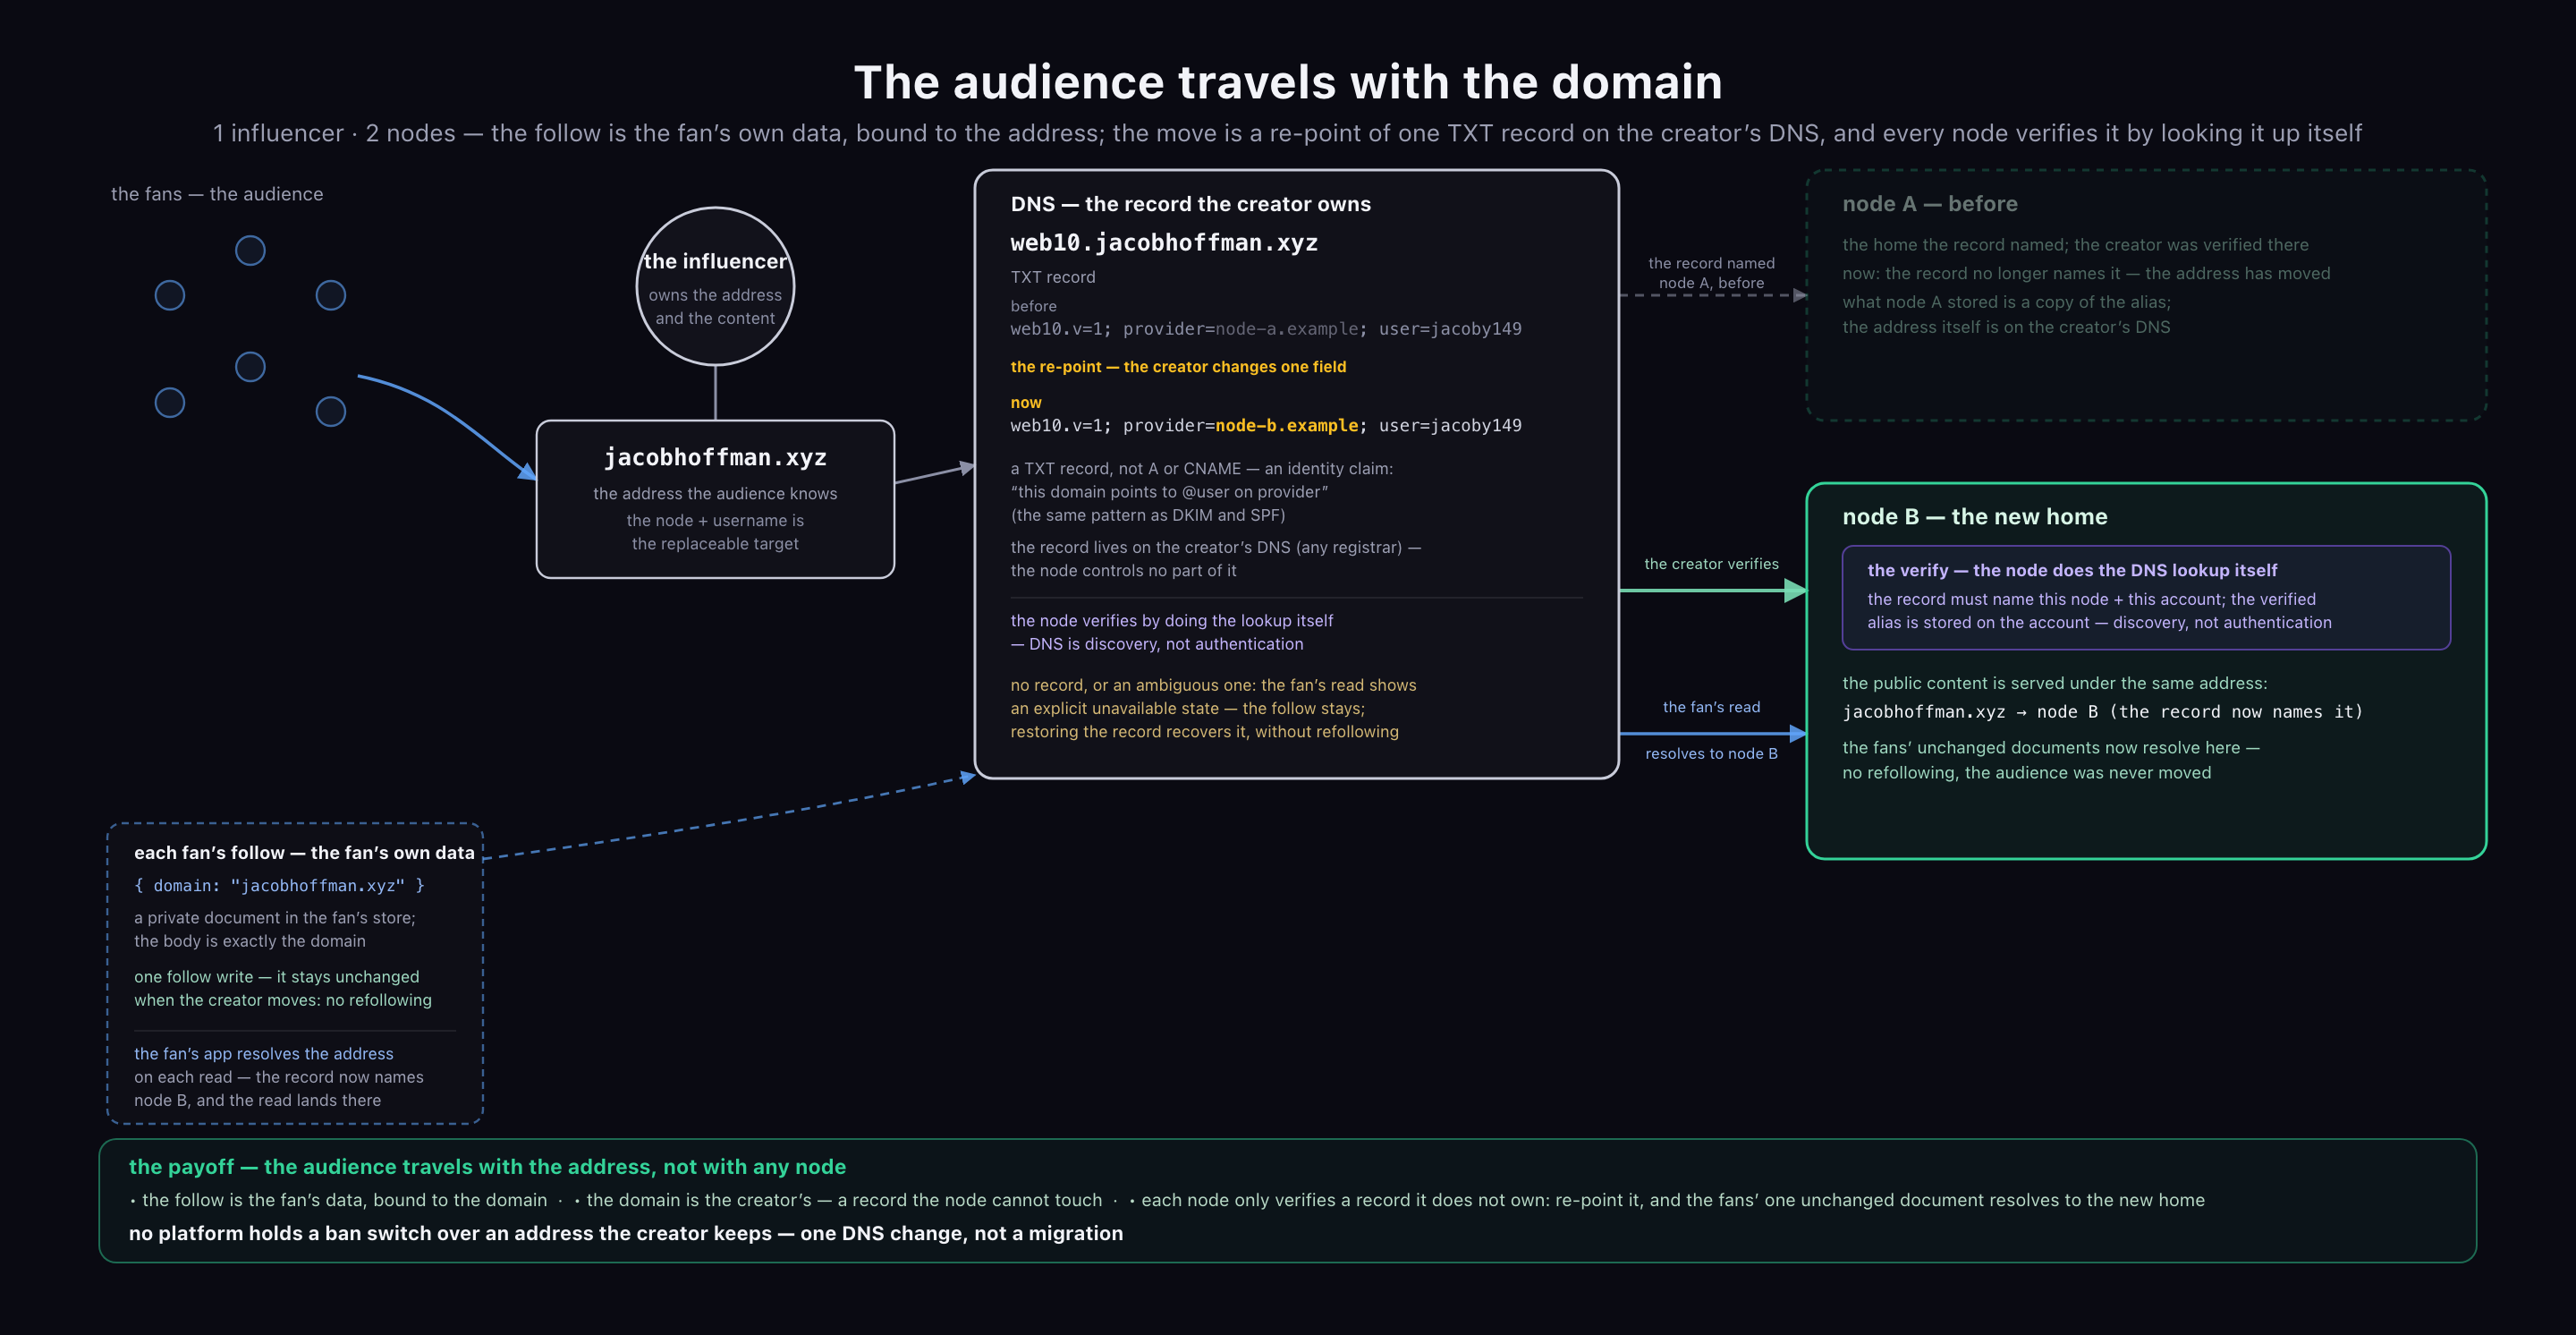
\includegraphics[width=\textwidth]{figs/fig-audience-portability.png}
\caption{The audience travels with the domain: one influencer, two nodes,
the DNS flip---the mechanism behind the demonstration of
\S\ref{sec:evidence}. The fans: each follow is the fan's own data---a
private document in the fan's store whose body is exactly the domain; one
follow write, unchanged when the creator moves; the fan's application
re-resolves the address on each read. The domain chip:
\texttt{jacobhoffman.xyz}---the address the audience knows; the node and
username are the replaceable target. The DNS card, shown in both states:
before \texttt{provider=node-a.example}, now
\texttt{provider=node-b.example}---one field changed. A TXT record, not an A
or CNAME record: an identity claim, the same pattern as DKIM and SPF; the
record lives on the creator's DNS, and the node controls no part of it. A
missing or ambiguous record gives an explicit unavailable state---the follow
stays, and restoring the record recovers it without refollowing. Node A
(faded): the home the record used to name; what it stored is a copy of the
alias. Node B (active): the verify gate---the node does the DNS lookup
itself, the record must name this node and this account, discovery not
authentication; the content is served under the same address, and the fans'
unchanged documents now resolve here. One DNS change, not a migration
(\S\ref{sec:network}).}
\label{fig:audience-portability}
\end{figure*}

%=============================================================================
\section{The money: the free web should have ads}
\label{sec:money}

Solid, Mastodon, and Bluesky ship no ad mechanism---ad-free by
conviction, a documented design property of each (\S\ref{sec:positioning})---
so on those platforms the creator's only revenue path is a cut the
platform takes, and the platform's leverage over the creator is
measurable: reach throttling, demonetization, deplatforming. web10 takes
the opposite position: the free web should have ads, and the ad
architecture matters. The position is on monetization, not on payment:
the node processes no payment and takes no cut of the creator's revenue.
It is on the rail that Figure~\ref{fig:monetization} draws.

Every application that writes into the store inherits the rail: a new ad
surface is a new query, not a new backend. web10-social builds the ad
catalog today; the snake game and the marketplace inherit it---any of
their documents can be a pinned ad target or a node ad. The node attaches
the ads at the boundary, checked the same way every other read is
checked (\S\ref{sec:boundary}), with the density split explicit: the
creator's layer is dense---the influencer's own offers, an affiliate
link, a sponsorship, the node's creator tier, land on roughly 80--90\%
of their content; the node's layer is sparse---the operator's overlay
lands on roughly 5--10\% of posts, node-controlled, default 10,
deterministic per reader, round-robin across the inventory. Both can be
present on the same post, and the node's overlay never suppresses the
creator's monetization. The inventory is tagged documents plus an offer
object---kind, the link that pays, call to action, disclosure---that the
platform never rewrites and never cloaks.

The money itself stays off-platform. The creator keeps 100\% of
affiliate and sponsor revenue: the link pays the creator, the platform
takes no cut and processes no payment. The node operator is a media
company: the overlay sells the node's own attention directly, and the
operator keeps the bulk of it---roughly 85--90\%. And because the overlay
density is node-controlled, nodes compete for the influencers by
lowering their rates. The horizon is a separate layer, not this system's
claim: an ad exchange, a payments rail, and the creator's own layout sit
ahead of it.

The market the rail makes is Figure~\ref{fig:node-market}. Because the
follow is the fan's own data, bound to the domain
(\S\ref{sec:network}), an influencer changing nodes is a rematch, not a
loss. Because the overlay density is node-controlled, the market between
influencers and nodes is a matching market on \emph{terms}---price, bans,
overlay, moderation style, with the self-hosted floor as the outside
option that keeps the prices honest. The three rents the paved platforms
hold over the creator---reach throttling, demonetization,
deplatforming; today's rent measured at one million subscribers, three
hundred thousand delivered---are structurally out. The competition is on
terms, not on leverage.

\begin{figure*}[t]
  \centering
  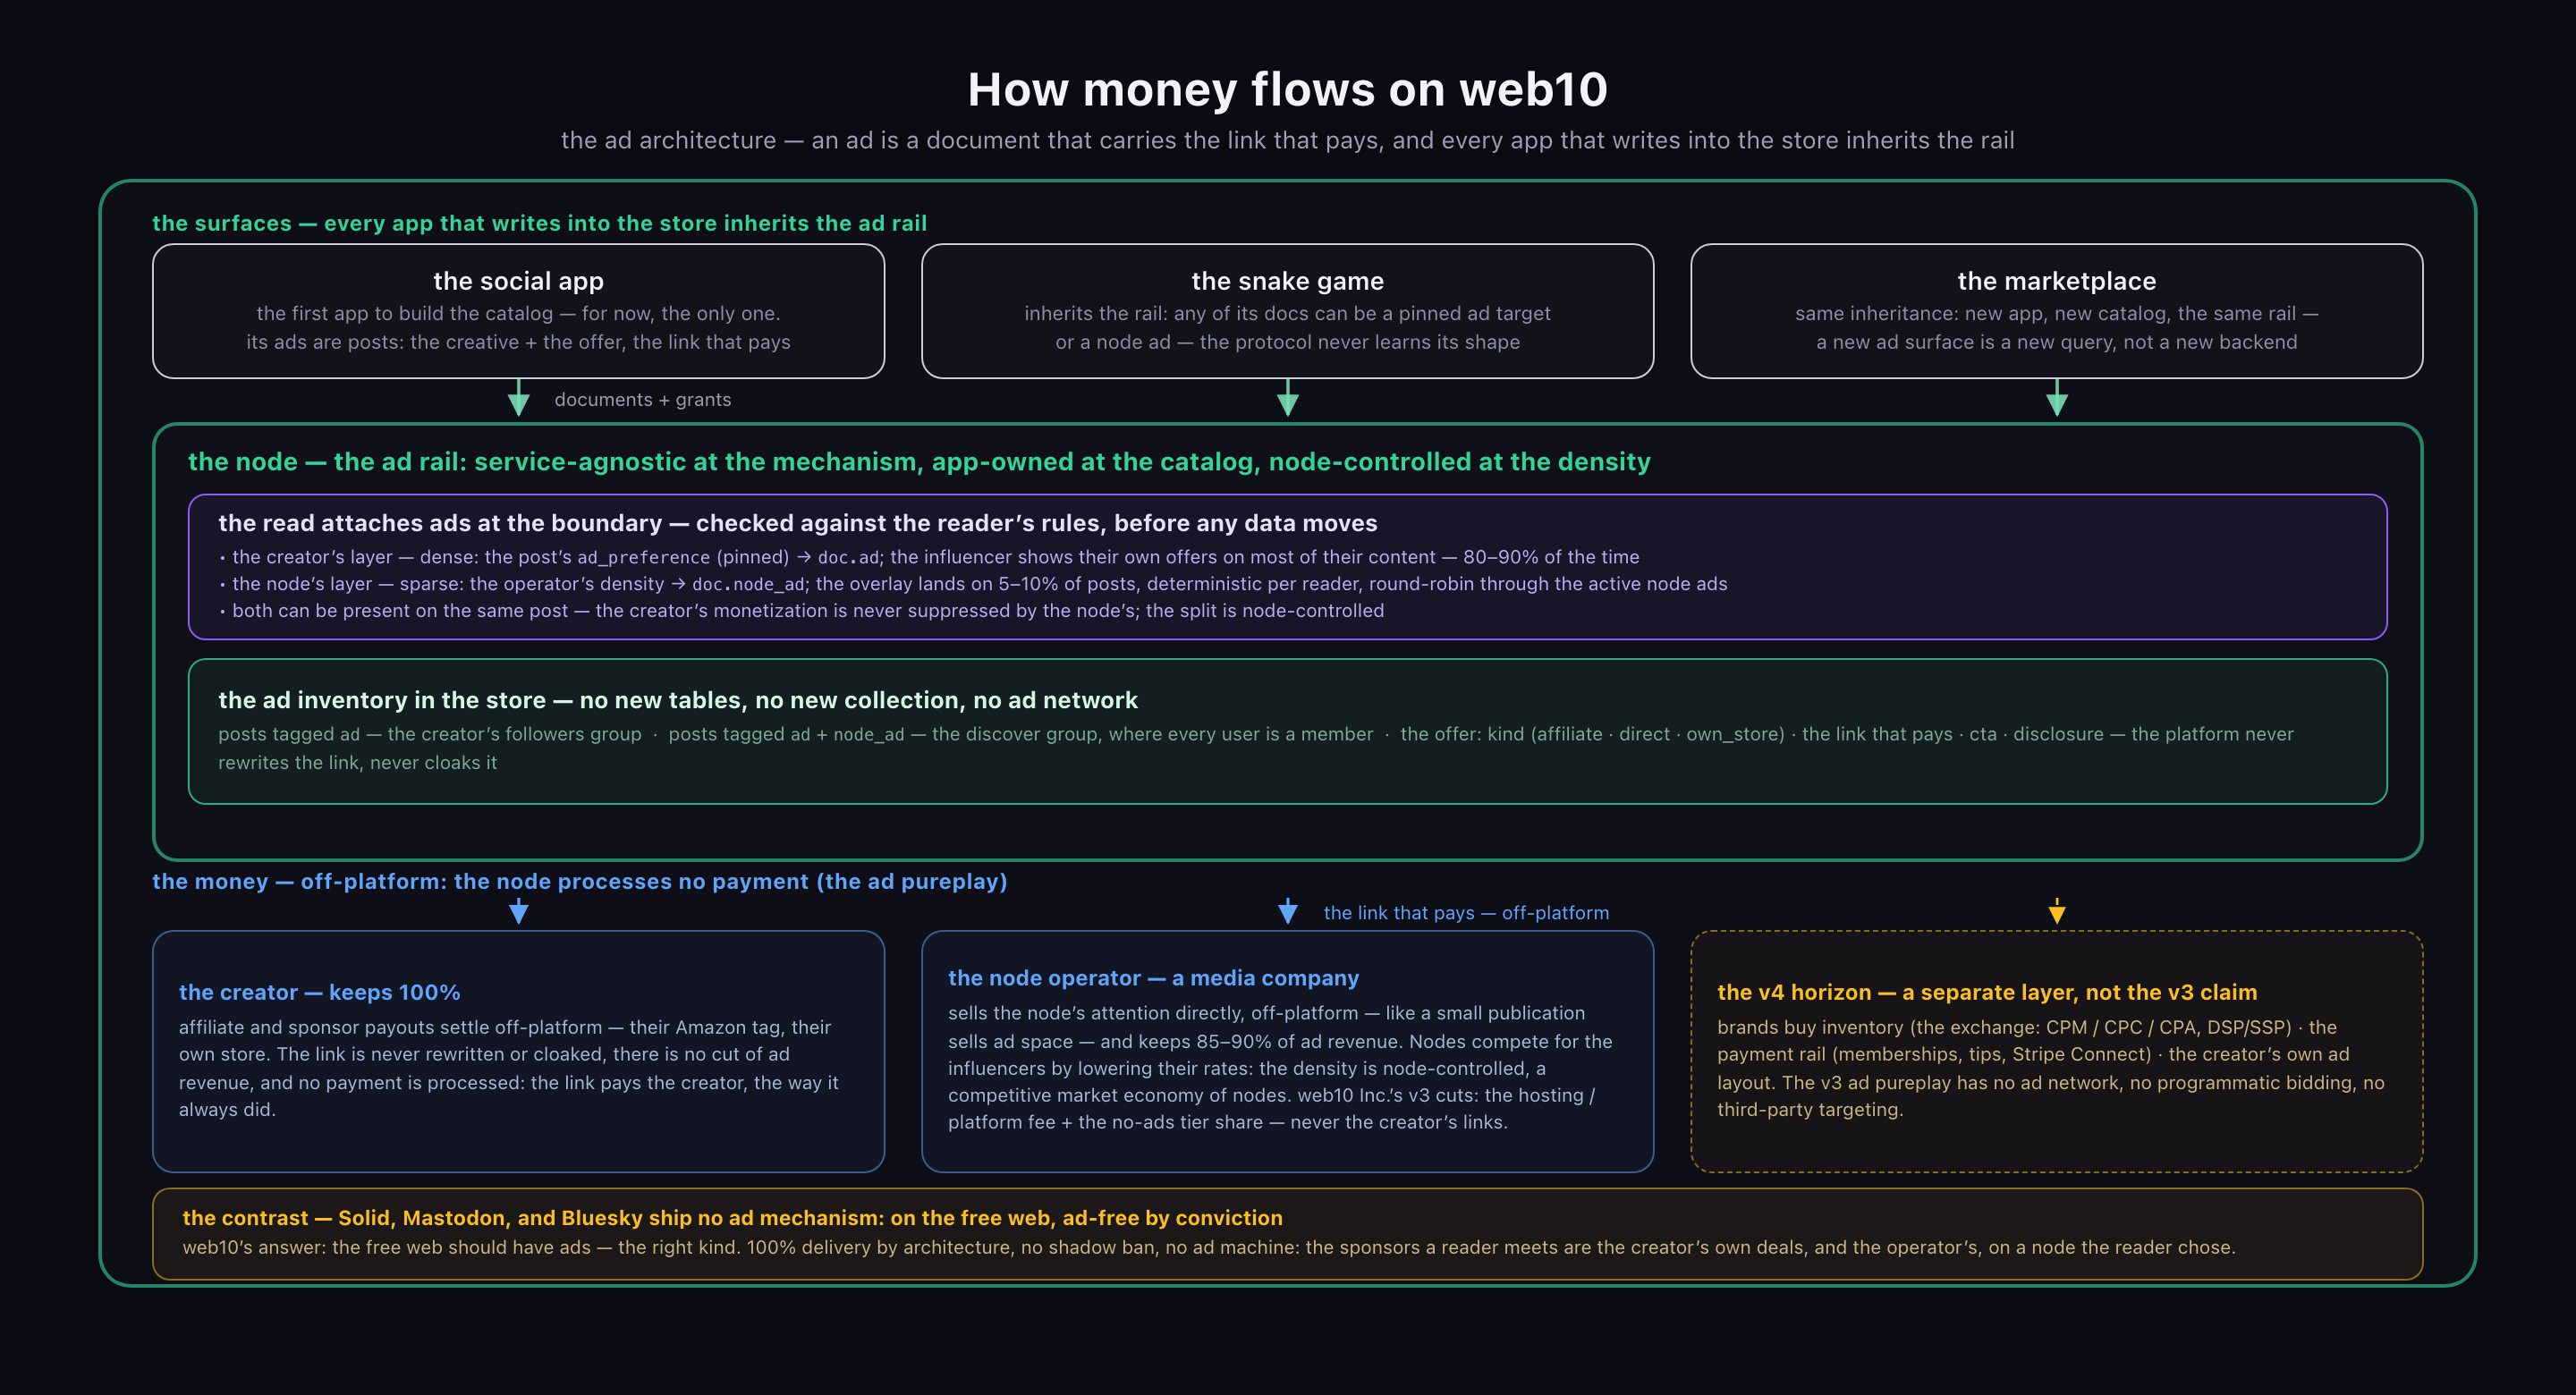
\includegraphics[width=\textwidth]{figs/fig-monetization.png}
  \caption{How money flows on web10---the ad rail. Top: every application
  that writes into the store inherits the rail---web10-social builds the
  catalog today; the snake game and the marketplace inherit it (a new ad
  surface is a new query, not a new backend). Middle: the node's rail---the
  boundary attaches the ads, checked the same way every other read is
  checked, with the density split explicit: the creator's layer dense
  (the influencer's own offers on roughly 80--90\% of their content) and the
  node's layer sparse (the operator's overlay on roughly 5--10\% of posts,
  node-controlled, default 10, deterministic per reader); both can be
  present on the same post, and the node's overlay never steals the
  creator's monetization. The inventory is tagged documents plus the offer
  object---kind, the link that pays, call to action, disclosure---never
  rewritten, never cloaked. Bottom: the money, off-platform---the creator
  keeps 100\% of affiliate and sponsor revenue (no cut of ad revenue, no
  payment processed); the node operator is a media company who sells the
  attention directly and keeps roughly 85--90\%, and nodes compete for the
  influencers by lowering their rates. The separate layer names the horizon
  (the exchange, the payments rail, the creator's own layout)---not this
  system's claim. The amber strip: Solid / Mastodon / Bluesky ship no ad
  mechanism---a documented design property; web10's answer: the free web
  should have ads.}
  \label{fig:monetization}
\end{figure*}

\begin{figure*}[t]
  \centering
  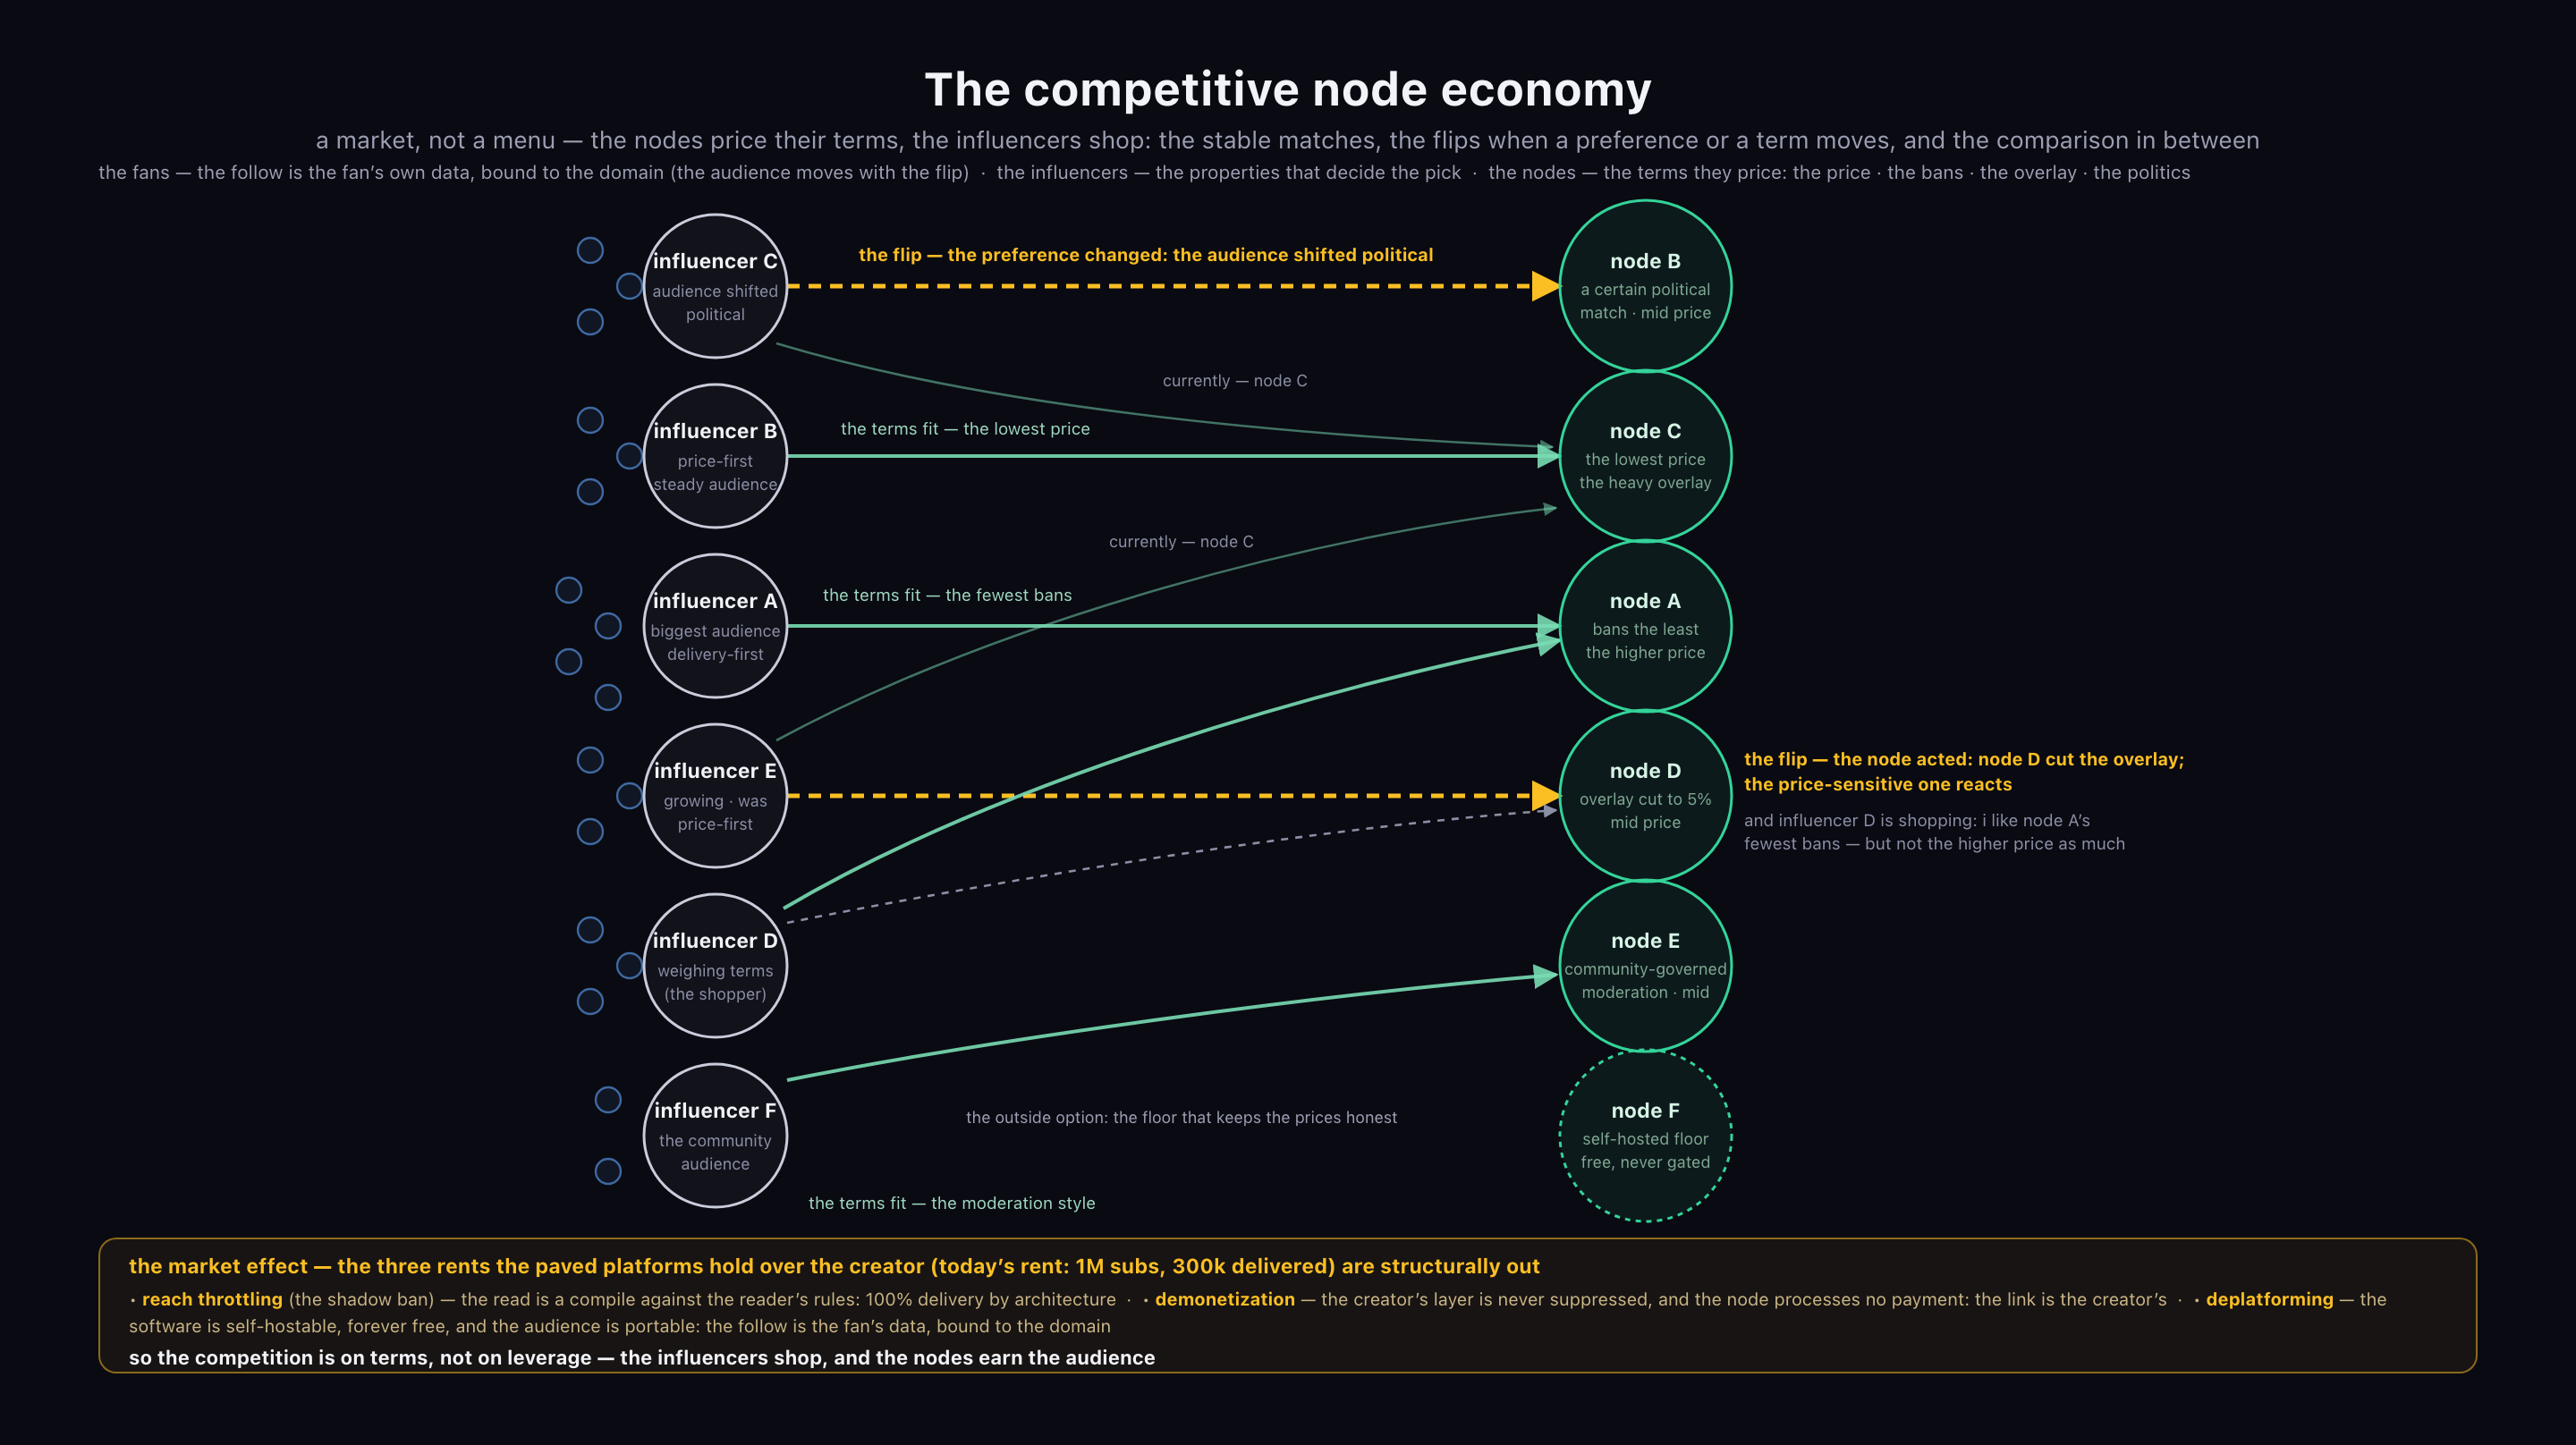
\includegraphics[width=\textwidth]{figs/fig-node-market.png}
  \caption{The competitive node economy: a matching graph, 6 $\times$ 6. Six
  influencers (left, neutral) matched against six nodes (right, green), each
  vertex carrying the market properties that decide the pick. The nodes
  price their own terms: A bans the least, the higher price $\cdot$ B a
  certain political match, mid price $\cdot$ C the lowest price, the heavy
  overlay $\cdot$ D the overlay cut to 5\%, mid price $\cdot$ E
  community-governed moderation, mid price $\cdot$ F the self-hosted floor---
  free, never gated, the isolated outside option that keeps the market's
  prices honest. The influencers carry their own properties (biggest
  audience / delivery-first $\cdot$ price-first $\cdot$ audience shifted
  political $\cdot$ the shopper $\cdot$ growing, was price-first $\cdot$ the
  community audience) with the fan dots by each: the follow is the fan's own
  data, bound to the domain---a flip is a rematch, not a loss. The edges
  carry the dynamics: the stable matches; two flips---one because the
  preference changed, one because the node acted; the shopping leg; and node
  C losing two of its three, because price alone does not hold the audience.
  The amber strip: the three rents the paved platforms hold over the
  creator---reach throttling, demonetization, deplatforming---structurally
  out; so the competition is on terms, not on leverage
  (\S\ref{sec:money}).}
  \label{fig:node-market}
\end{figure*}

%=============================================================================
\section{Lessons from running it}
\label{sec:lessons}

The industry track asks what running a system taught that designing it
did not. Three things, in roughly the order they bit.

\subsection{The node keeps resisting the killer app}

The platform's hardest dependency is its own killer app, and the killer
app always asks for bespoke surface: a feed is faster to ship as an
endpoint than as a client query; a group's name, description, and banner
photo look like exactly the kind of thing a \texttt{group\_identity}
table would hold; a session oracle that knows about the followers group
would make the social app's re-authentication path trivial. Four such
node surfaces were built, and all four were removed: the dedicated feed
endpoint (replaced by an application-written query over the services it
composes), the group-identity table with its own endpoint (replaced by
documents in an app-named service read through the normal CRUD and grant
path), the followers-group check inside the generic session oracle
(moved to the one application that knows what a followers group is),
and an ad path that hard-coded a collection name (replaced with a tag
and group membership the applications themselves manage). The test that
caught each one is one sentence: \emph{would a notes app, a music app,
or a shop use this endpoint?} The cost of holding the line is real and
visible---the client does more work---and the payoff is
\S\ref{sec:extend}: a game and a marketplace with no relationship to
the social application's code, reading its profiles through the same
boundary, no node change when either appeared.

\subsection{A self-healing schema raced its own readers}

On a fresh stack, the node self-heals its metadata schema with a
deferred \texttt{ALTER TABLE} at boot, adding columns to
\texttt{group\_contracts} that older databases lack. An early read that
lands before the \texttt{ALTER} commits fails with an
unknown-identifier error, and it is easiest to hit exactly where the
stack is newest: a clean database, a cold boot, the first request.
The lesson: the schema additions must land synchronously and be
guaranteed before the first read of that table, or the columns must
exist at table creation---and the regression that guards it boots a
fresh database and immediately reads the table. The
general lesson is the one that survives the particular bug: a
self-heal that may lag is fine; a self-heal that may \emph{race} is
not. Test the fresh-boot path, not just the steady state.

\subsection{What the shared columnar table costs, day to day}

The data-plane choice of \S\ref{sec:store} trades physical isolation
for cross-author composition, and the running platform meets the price
of that trade every day. Every read pays the version deduplication,
because \texttt{ReplacingMergeTree} settles versions only when it
merges. ``Deletion'' is an insert, so a tombstone is a row that must be
ranked, not discarded. Merge pressure is background CPU that does not
show up in request latency until the host is busy. Point queries are
paid to an engine built for scans. And every tenant in the node shares
the same resources. These are not defects of the design; they are the
design's operating envelope---and they are the reason
reader isolation lives at the query boundary of \S\ref{sec:boundary},
not in a physical partition.

%=============================================================================
\section{The evidence}
\label{sec:evidence}

The evidence is connected, bounded, and named; each part is organized as
the question it answers. Does an unrelated application actually reuse
another's data through the access boundary, with consent and revocation
exercised in a real browser (\S\ref{sec:ev-interop})? Does a grant reach
across the node boundary, and can the owner revoke it locally
(\S\ref{sec:ev-federation})? Does a public subscription outlive its
provider (\S\ref{sec:ev-domain})? What does the access layer cost
(\S\ref{sec:ev-fanout})? And is anyone actually using this
(\S\ref{sec:ev-operating})? The first four are synthetic data on
isolated test stacks; the operating point is a read-only observation of
the production node. None is a capacity or scale result.

\subsection{Does an unrelated application actually reuse another's data?}
\label{sec:ev-interop}

A fresh account logged into web10-social through its authenticator popup
and edited its profile name to Alex Morgan. The browser approved Snake's
app request; the player earned and saved ten points, and the leaderboard
displayed the joined profile. After app-contract revocation, a new query
returned 403 and the leaderboard cleared the result and displayed an
access error. After sign-out, Marketplace requested its service
permission through the popup, published a listing, and displayed the same
profile; reloading the listing's detail URL preserved the result. API
assertions checked exact authors, row counts, profile bodies, and
listing identity, so the username fallback alone could not satisfy the
test.

A separate HTTP case with three accounts and two social-written profiles
checked the exact two-author joins: with no app permission for
\texttt{profile} both queries were denied; granting it enabled the joins;
revoking the app contract denied them again. A separately labeled
private-profile fixture isolated the group gate: membership enabled an
exact inner join; removal emptied it while the scores remained readable.

All three cases---desktop at 1440 pixels, mobile at 375 pixels, and HTTP
correctness---passed in the final fresh-stack run on 2 November 2026,
with zero retries or skips. The run used a four-vCPU, 8-GB DigitalOcean
sfo2 host with ClickHouse 24.8.14.39, Playwright 1.63.0, and Chromium
153; the exact source, configuration, image identities, results, and all
16 original captures are retained in
\domainartifactdir{research/interoperability-demo}{the
interoperability artifact}. The hosted apps share one browser origin,
although the HTTP case supplies a separate app Origin: these controls
establish named grant/revocation behavior across applications, not
separate-origin isolation or an independently recruited developer study,
and they establish behavior, not a stale-access or capability-expiry
bound.

\subsection{Does a grant reach across the node boundary---and can the
owner revoke it locally?}
\label{sec:ev-federation}

Two API processes, separate ClickHouse and MinIO instances,
independently generated HS256 signing secrets, and real HTTPS
home-issuer certification with an ephemeral test CA. Bob creates a
private group and document through B's API. Alice's A-issued JWT
initially fails both B's document read and B's query---and giving a
\emph{distinct B-side Alice} the membership also fails to authorize
A's Alice: two Alices, same name, told apart only through the qualified
principal. Bob then grants the exact foreign principal through the owner
API; both read paths return the exact document; removing that
membership denies both; regrant restores both.

All steps reused the same JWT, and the certification traffic shows why
the model works the way \S\ref{sec:network} states it: A's TLS proxy
records exactly \emph{one} successful certification across the entire
lifecycle, while B rechecks access on every read. A foreign-provider JWT
signed with B's key is rejected twice, with one failed issuer call and a
negatively cached second rejection; an independent Origin-bearing query
gate denies a local namesake's app grant, allows a qualified foreign
fixture, and denies again after its revocation. The scenario completed
without retries on an unmodified source snapshot; exact source,
configuration, request outcomes, image identities, and cleanup records
are retained in \domainartifactdir{research/federation-demo}{the
experiment artifact}. This is a correctness experiment, not a deployment
or load trial: the test CA and Docker-internal addresses do not
establish public-internet interoperability, and owner grant/removal is
not foreign self-join.

\subsection{Can a public subscription outlive the provider that hosts it?}
\label{sec:ev-domain}

A separate research client stores only the creator's normalized domain in
a private app document at the reader's independent home. It freshly
resolves the existing TXT pointer, checks the selected account's verified
alias, and reads public posts anonymously---through ordinary CRUD and
groups and the existing authenticated domain-verification endpoint, not a
new node follow API.

On desktop (1440\,$\times$\,1000) and mobile (375\,$\times$\,812), the
creator logged in, published the TXT record, and verified the old account
through actual local UDP DNS; the reader clicked Follow once. Then the
old API and TLS services were stopped. With the original provider
unavailable, the creator re-pointed DNS and verified a new account without
the old provider's approval. Reload and ordinary reader login displayed
new public posts with the identical stored follow ID and body, and one
total follow creation; no old content was migrated. And the asymmetry
that should hold: explicit old private access returned 200 while
new-target private access remained 403---the public subscription follows
the domain, but private access is not inherited by the new target.
Figure~\ref{fig:audience-portability} draws the move; the exact panel
captures, the authenticated hookup, and the 375px evidence remain in the
artifact.

Controls delayed real responses at five identity-transition boundaries
and verified that logout or account changes prevented stale UI updates;
missing or ambiguous DNS cleared displayed content without deleting the
saved subscription; and the DNS/alias/public requests carried no
credentials. Exact source and configuration, ten captures, request
outcomes, and cleanup records are retained in
\domainartifactdir{research/domain-portability-demo}{the
prototype artifact}. This is a configured two-node client, not deployed
social follows or private principal continuity: domain control, resolver
availability, and the availability of the reader's home and new provider
are assumptions rather than guarantees; domain sale, theft, and expiry
are not solved; and the result demonstrates bounded public subscription
continuity, not absolute unbannability.

\subsection{What does the access layer cost, and where does the cost live?}
\label{sec:ev-fanout}

The read path resolves the reader's readable groups before the query
executes. We measured that cost to understand the design, not to report
a latency distribution: the question was whether per-group metadata
resolution scales with the number of candidate groups, and what batched
resolution buys. Figure~\ref{fig:k1000-curve} plots the trial; the
numbers it carries are stated here, with the scope that bounds them.

\textbf{Setup.} One sequential trial on a DigitalOcean sfo2
\texttt{s-4vcpu-8gb} host (four vCPUs, 8\,GB nominal RAM, Ubuntu 24.04,
Linux 6.8, Docker 29.1.3), co-locating a single Uvicorn process and
ClickHouse 24.3.18.7. The synthetic seed (seed 42) created 1,000
creators with one small post each and a reader who joined all their
groups; those groups also granted public reads. Personal queries supplied
$K=10$, $100$, or $1{,}000$ candidate groups on this same dataset and
host; a separate discover query supplied one board group ($K=1$),
containing ten additional posts. Twenty samples per cell, 400
measurements; all 320 HTTP requests returned 200. The queries selected
document IDs and bodies, ordered by creation time and ID, with a limit of
20; they did not execute engagement joins, media preparation, or browser
page assembly, and they supplied no Origin header, so this trial does not
exercise the browser-origin app-contract gate.

\textbf{Variants.} The per-group resolver performs point metadata queries
for each candidate group. The batched resolver fetches memberships,
principal-class grants, and role definitions across the candidate set in
three database queries, then resolves access in memory. We measured each
resolver with real document execution (B) and a fixed 20-row synthetic
scan result (C); C retains the policy/compilation path but is not an
output-equivalent execution. A third variant (A) precompiles the
known-readable projection and times ClickHouse execution directly,
outside the HTTP handler.

\textbf{Finding.} The per-group resolver's cost grows linearly with the
number of candidate groups: increasing $K$ from 10 to 1,000 increased
median readable time $100.44\times$ (75.03\,ms to 7,535.71\,ms; p95
93.30\,ms to 8,504.61\,ms), against $9.12\times$ for the batched
resolver (23.47\,ms to 213.98\,ms; p95 31.17\,ms to 284.03\,ms). At
$K=1000$ the batched path is $35.22\times$ faster on readable time and
$21.04\times$ faster on handler time (363.31\,ms median handler). Stubbing
the execution keeps the separation: 8,388.39\,ms per-group versus
222.57\,ms batched at $K=1{,}000$. The per-group path still completes
requests, but its 7.64-second median at $K=1000$ is a practical
bottleneck for a reader who follows many creators; the batched path's
363\,ms is not. The direct-scan baseline stayed at 28.6--54.2\,ms across
$K = 10$--$1{,}000$: the document scan was already done while the access
layer was still resolving. This is the design decision the measurement
drives: the query endpoint should use the batched resolver for large
candidate sets.

The tradeoff is honest in both directions. Batching is not uniformly
cheaper: at the discover board's $K=1$, the per-group path is faster
(9.53\,ms readable versus 25.37\,ms batched), because three fixed round
trips dominate when there is one group to check. And batching does not
make the cost constant: the batched handler median still grew
$4.47\times$ over the 100-fold increase in $K$, as the metadata to
process and the compiled query to emit both grow with the candidate set.
The trial is a single sequential run on a simplified projection; it
characterizes the access layer's cost structure---metadata fan-out is
the dominant term at large $K$, and batching is the mitigation---and does
not establish a latency distribution, a capacity bound, or a causal
authorization-overhead estimate; $B - A$ is a pipeline-versus-scan
comparison, not a matched causal measurement. Exact source, configuration,
and per-sample measurements are retained in
\domainartifactdir{research/experiments/costfn}{the measurement
artifact}; an earlier 100-creator trial on a different host showed the
same qualitative tradeoff and is not pooled with this trial.

\begin{figure*}[t]
  \centering
  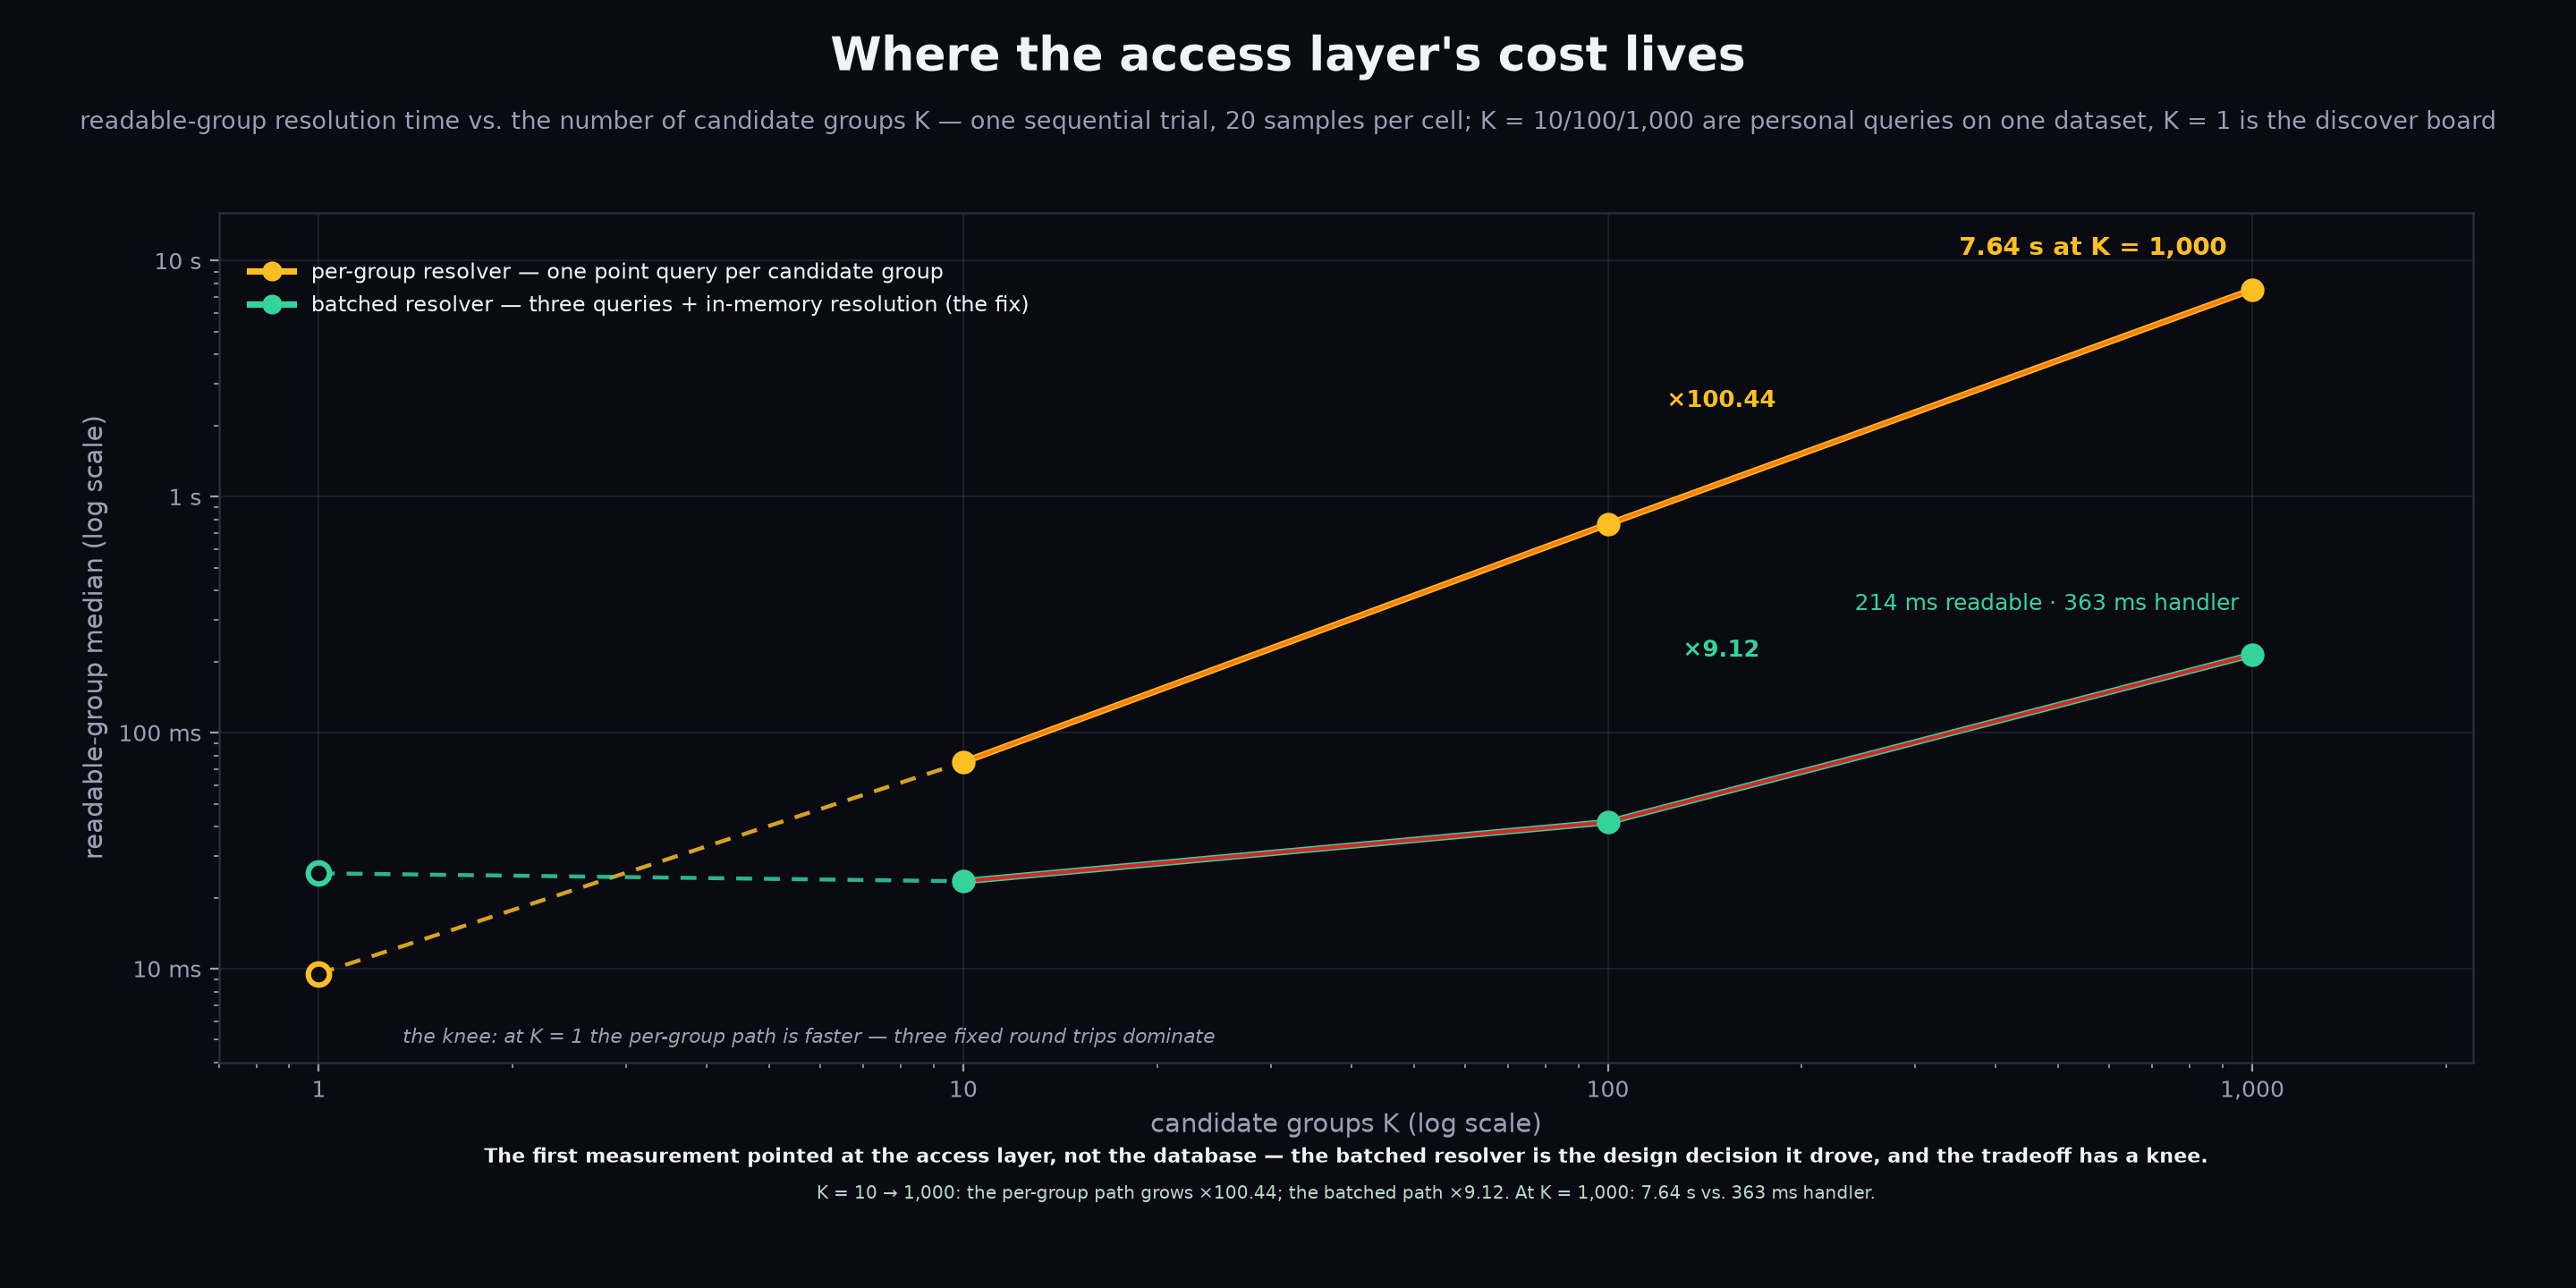
\includegraphics[width=\textwidth]{figs/fig-k1000-curve.png}
  \caption{Where the access layer's cost lives: readable-group resolution
  time versus the number of candidate groups $K$ (log-log), the trial of
  \S\ref{sec:ev-fanout}. The per-group resolver (amber) grows $\times$100.44
  over $K = 10 \rightarrow 1{,}000$ and reaches 7.64\,s at $K = 1{,}000$;
  the batched resolver (green) grows $\times$9.12 and sits at 214\,ms
  readable (363\,ms handler). $K = 1$ is the discover board---one candidate
  group, an open marker on the dashed leg---where the per-group path is
  faster, because three fixed round trips dominate. The knee is the tradeoff;
  the batched resolver is the design decision the measurement drove
  (\S\ref{sec:ev-fanout}).}
  \label{fig:k1000-curve}
\end{figure*}

\subsection{Is anyone actually using this?}
\label{sec:ev-operating}

The platform is deployed and serving authenticated users. A read-only
observation of the production node on 28 October 2026 recorded 597
account rows, 593 live documents across 30 distinct authors and 10
services, 49 group contracts, and 1,298 membership rows, on a host
running the social, authenticator, and API frontends. Nine authenticated
browser navigations (following feed, music, groups) returned HTTP 200
with a retained session and zero uncaught page errors; the following feed
rendered 20 posts in a median 5,396\,ms of full-page readiness. This is
an operating point---evidence the system runs and serves real users---not
a capacity or scale result: the host also runs a development stack, the
observation is a snapshot without an activity window, and the readiness
figure includes frontend startup and network work, not server-query
duration. The 5.4-second figure is the kind of number the industry track
exists to report: it is real, it is bad enough to matter, and the
full-feed dissection named in \S\ref{sec:concl} is the measurement it
asks for.

%=============================================================================
\section{No new part, one combination}
\label{sec:positioning}

The contribution is an integration of established ideas: user-addressed
storage, user-managed grants, and application-defined queries over
authorized relations. The two comparison figures of
\S\ref{sec:store} and \S\ref{sec:extend} organize the matchup visually;
what follows is positioning, not a survey. We discuss design differences
from the cited systems rather than claiming that no prior implementation
combines these capabilities.

\textbf{Solid: the closest prior work.}
Solid~\cite{solid2016} separates applications from personal data stores
(pods), with social application work~\cite{solid-apps2016} and a
maintained Community Solid Server~\cite{css2024}. WAC supports resource
permissions and group agents through
\texttt{acl:agentGroup}~\cite{wac2022}, and ACP adds agent, client, and
issuer matching with allow/deny mode sets~\cite{acp2022}---web10 does
not claim Solid lacks group or client authorization; it has both. The
distinction is in the \emph{shape} of the model: Solid's access control
is resource-centric---ACLs attached to linked-data resources, evaluated
per resource---while web10's is service-centric: a uniform
principal-class $\times$ service $\times$ operation vocabulary in which
the grant is a row naming a globally addressable principal, exposed to
the end user rather than an infrastructure operator. And the query
surface: Solid's cross-pod query cost depends on deployment, caching, and
linked-data traversal; web10 composes application-defined SQL over a
shared columnar store with the access decision made on the input
(\S\ref{sec:boundary})---the fork of Figure~\ref{fig:composition}. A
performance comparison would require a matched workload and deployment;
we do not claim one here.

\textbf{Federation: the content moved, the access layer did not.}
ActivityPub~\cite{activitypub2018} (Mastodon) defines federated
server/server activity delivery; its authorization is
platform-defined---follow/block and collection-level visibility---not
per-principal grants over application-defined services.
ATProto~\cite{kleppmann2024} (Bluesky) separates repositories, relays,
and AppViews, supporting user agency and provider switching; its
delegation is app-to-user-data---per-collection, per-action permissions
over the user's own repo---and its read path is the platform's fixed
endpoints or a record the app has replicated into its own database.
Neither has a shared store to compose across, and neither lets a second
application hold a typed read on the first application's data. web10's
seam is the one Figure~\ref{fig:platforms} draws: service-scoped,
user-managed grants, and application-defined queries over the resulting
authorized relations---the seam \S\ref{sec:extend} exercises with two
applications that share nothing but the document convention.

\textbf{The columnar boundary: the placement the OLTP answer did not
make.} The tenant-isolation literature---shared tables with an
organization identifier (Force.com~\cite{force2009}), schema
mapping~\cite{aulbach2008}, the shared-versus-separate
spectrum~\cite{jacobs2007}---is the closest systems ancestor, with the
tenant at the organization; web10's key-space per user takes that
spectrum to its limit (\S\ref{sec:store}). PostgreSQL row-security
policies~\cite{postgres-rls} are the alternative enforcement location:
per-row policy evaluation inside the engine. At industrial scale,
Zanzibar~\cite{zanzibar2019} is the closest prior art in
relationship-based authorization: a uniform ACL data model across
hundreds of services, with consistency as a first-class problem---but
the model is infrastructure-side: the operator defines the relationship
schema and the service enforces it. web10 exposes service-scoped grants
as user-managed data, names globally addressable principals, and enforces
access at the query layer over a shared columnar store. TAO~\cite{tao2013}
is the deployed precedent for read-time checking at social-graph scale
(a billion reads per second, the privacy check per item, pull not push):
web10's boundary is the same idea---every row access-checked on its way
out---applied to service-namespaced documents in a columnar store, with
the check expressed as a reader-filtered CTE compiled in before the
caller's aggregation runs, rather than a per-item predicate. The matched
policy-and-workload comparison of these placements is the forward scope
\S\ref{sec:ev-fanout} leaves to run.

\textbf{Monetization: the gap the free-web camp shipped deliberately.}
Solid, Mastodon, and Bluesky ship no ad mechanism. That is a documented
design property of each---the free-web camp---not an oversight, and on
those platforms the creator's revenue path is the platform's cut, with
the rent measurable: reach throttling, demonetization, deplatforming.
web10's answer is the ad rail of \S\ref{sec:money}: the creator keeps
100\% of affiliate and sponsor revenue, the node operator is a media
company that sells the node's own attention, and the platform takes no
cut and processes no payment---and the market the rail makes is
Figure~\ref{fig:node-market}, where the competition is on terms, not on
leverage.

%=============================================================================
\section{Conclusion}
\label{sec:concl}

What makes your data worth owning is the graph around it: who follows
you, who belongs where, who may read what. No platform lets you keep that
graph---the content is portable in principle, and the permissions are
the part that stays. web10 is the generalization that changes it: a
user-addressed network in which applications define their own document
services over a shared columnar store in each sovereign node, in which a
uniform, user-managed access model lets any principal on any node hold a
role in a user's groups, and in which the query layer supplies the
reader's service relations before joins and aggregation execute.

The evidence is connected, bounded, and named. A game and a marketplace
reuse the social application's profiles with no node change and no API
agreement, with browser consent and cross-author controls exercised end
to end; a two-node experiment shows a foreign principal granted, reading,
revoked, and restored under a single cached certification; a browser
prototype keeps a public subscription alive after its provider goes
dark---while the private grants correctly stay behind. And the metadata
fan-out measurement identifies where the access layer's cost actually
lives at scale: at 1,000 candidate groups, batching reduced median
handler time from 7.64\,s to 363\,ms, while costing more at one group.
This is a design decision, not a scalability claim---and it is the kind
of concrete, measured tradeoff an operating system earns.

The generic core was earned, not designed from the top: the four
built-and-deleted node surfaces of \S\ref{sec:access} are the visible
part. And the market the data plane makes is why the reach is worth it:
the creator keeps their own monetization, and the nodes compete for the
creators on terms, not on leverage.

The forward scope is specific: federation beyond the isolated
correctness slice (\S\ref{sec:ev-federation}), full-feed and concurrent
workload measurements, a matched shared-table policy baseline
(\S\ref{sec:ev-fanout}), and revocation-latency bounds. The architectural
contribution is the integration itself.

Email let the data leave the building. web10 lets the permissions leave
it too.

%=============================================================================
\bibliographystyle{ACM-Reference-Format}
\bibliography{../references/web10-references}

\end{document}
